\chapter{Search}
In this chapter we discuss various \emph{\color{blue}search algorithms}.  First, we define
the notion of a \emph{\color{blue}search problem}.  As one of the examples, we will discuss the
\href{https://en.wikipedia.org/wiki/15_puzzle}{sliding puzzle}.  Then we 
introduce various algorithms for solving search problems.  In particular, we present
\begin{enumerate}
\item breadth first search,
\item depth first search,
\item iterative deepening,
\item bidirectional breadth first search,
\item $\mathrm{A}^*$ search, 
\item bidirectional $\mathrm{A}^*$ search,
\item iterative deepening $\mathrm{A}^*$ search, and
\item $\mathrm{A}^*$-$\mathrm{IDA}^*$ search.
\end{enumerate}

\begin{Definition}[Search Problem]
  A \emph{\color{blue}search problem} is a tuple of the form
  \\[0.2cm]
  \hspace*{1.3cm}
  $\mathcal{P} = \langle Q,\mathtt{nextStates}, \mathtt{start}, \mathtt{goal}\rangle$
  \\[0.2cm]
  where
  \begin{enumerate}
  \item $Q$ is the set of states, also known as the \emph{\color{blue}state space}.
  \item $\texttt{nextStates}$ is a function taking a state as input and returning the set of those
        states that can be reached from the given state in one step,
        i.e.~we have
        \\[0.2cm]
        \hspace*{1.3cm}
        $\texttt{nextState}:S \rightarrow 2^S$.
        \\[0.2cm]
        The function \texttt{nextState} gives rise to the \emph{\color{blue}transition relation} $R$, which is a
        relation on $Q$, i.e.~$R \subseteq Q \times Q$.  This relation is defined as follows:
        \\[0.2cm]
        \hspace*{1.3cm}
        $R := \bigl\{ \pair(s_1, s_2) \in Q \times Q \mid s_2 \in \mathtt{nextState}(s_1) \bigr\}$.
        \\[0.2cm]
        If either $\pair(s_1, s_2) \in R$ or $\pair(s_2, s_1) \in R$, then  $s_1$ and $s_2$ are
        called \emph{\color{blue}neighboring states}.
  \item $\mathtt{start}$ is the \emph{\color{blue}start state}, hence $\mathtt{start} \in Q$. 
  \item $\mathtt{goal}$ is the \emph{\color{blue}goal state}, hence $\mathtt{goal} \in Q$.

        Sometimes, instead of a single $\mathtt{goal}$ there is a set of goal states $G$.
  \end{enumerate}
  A \emph{\color{blue}path} is a list $[s_1, \cdots, s_n]$ such that $\pair(s_i, s_{i+1}) \in R$ for all $i \in
  \{1,\cdots,n-1\}$. 
  The \emph{\color{blue}length} of this path is defined as the length of the list. 
  A path $[s_1, \cdots, s_n]$ is a \emph{\color{blue}solution} to the search problem $P$ iff the following
  conditions are satisfied:
  \begin{enumerate}
  \item $s_1 = \mathtt{start}$, i.e.~the first element of the path is the start state.
  \item $s_n = \mathtt{goal}$, i.e.~the last element of the path is the goal state. 
  \end{enumerate}
  A path $p = [s_1, \cdots, s_n]$ is a \emph{\color{blue}minimal solution} to the search problem $\mathcal{P}$ iff it is a
  solution and, furthermore, the length of $p$ is minimal among all other solutions. \eoxs
\end{Definition}

\remark
In the literature, a \emph{\color{blue}state} is often called a \emph{\color{blue}node}.  In these lecture
notes, I will also refer to states as nodes.  \eoxs

\example
We illustrate the notion of a search problem with the following example, which is also known as the 
\href{https://en.wikipedia.org/wiki/Missionaries_and_cannibals_problem}{missionaries and cannibals problem}: 
Three missionaries and three infidels have to cross a river that runs from the west to the east.
Initially, they are on the northern shore.  There is just one small boat and that boat has only room
for at most two passengers.  Both the missionaries and the infidels can steer the boat.  However, if
at any time the missionaries are confronted with a majority of infidels on either shore of the
river, then the missionaries have a problem.  

\begin{figure}[!ht]
\centering
\begin{Verbatim}[ frame         = lines, 
                  framesep      = 0.3cm, 
                  firstnumber   = 1,
                  labelposition = bottomline,
                  numbers       = left,
                  numbersep     = -0.2cm,
                  xleftmargin   = 0.8cm,
                  xrightmargin  = 0.8cm,
                ]
    problem := [m, i] |-> m > 0 && m < i;

    noProblemAtAll := [m, i] |-> !problem(m, i) && !problem(3 - m, 3 - i);

    nextStates := procedure(s) {
        [m, i, b] := s;
        if (b == 1) {  // The boat is on the northern shore.
            return { [m - mb, i - ib, 0]
                   : mb in {0 .. m}, ib in {0 .. i}           
                   | mb + ib in {1, 2} && noProblemAtAll(m - mb, i - ib)
                   };
        } else {
            return { [m + mb, i + ib, 1]
                   : mb in {0 .. 3 - m}, ib in {0 .. 3 - i}           
                   | mb + ib in {1, 2} && noProblemAtAll(m + mb, i + ib)
                   };
        }
    };
    start := [3, 3, 1];
    goal  := [0, 0, 0];
\end{Verbatim}
\vspace*{-0.3cm}
\caption{The missionary and cannibals problem codes as a search problem.}
\label{fig:missionaries.stlx}
\end{figure}
\noindent
Figure \ref{fig:missionaries.stlx} shows a formalization of the missionaries and cannibals problem
as a search problem.  We discuss this formalization line be line.
\begin{enumerate}
\item Line 1 defines the auxiliary function \texttt{problem}.

      If $m$ is the number of missionaries on a given shore, while $i$ is the number of infidels on
      that same shore, then $\textsl{problem}(m, i)$ is \texttt{true} iff the missionaries have a problem on that
      shore.  
\item Line 3 defines the auxiliary function \texttt{noProblemAtAll}.  

      If $m$ is the number of missionaries on the northern shore and $i$ is the number of infidels on
      that shore, then the expression $\texttt{noProblemAtAll}(m, i)$ is true, if there is no problem
      for the missionaries on either shore.  

      The implementation of this function uses the fact that if $m$ is the number of missionaries on
      the northern shore, then $3-m$ is the number of missionaries on the southern shore.  Similarly,
      if $i$ is the number of infidels on the northern shore, then the number of infidels on the
      southern shore is $3 - i$.
\item Line 5 to 18 define the function \texttt{nextStates}.  A state $s$ is represented as a triple of
      the form
      \\[0.2cm]
      \hspace*{1.3cm}
      $s = [m, i, b]$ \quad where $m \in \{0,1,2,3\}$, $i \in \{0,1,2,3\}$, $b \in\{0,1\}$.
      \\[0.2cm]
      Here $m$ is the number of missionaries on the northern shore, $i$ is the number of infidels on
      the northern shore, and $b$ is the number of boats on the northern shore.
      \begin{enumerate}[(a)]
      \item Line 6 extracts the components $m$, $i$, and $b$ from the state $s$.
      \item Line 7 checks whether the boat is on the northern shore.
      \item If this is the case,  then the states reachable from the given state $s$ are those
            states where $\mathtt{mb}$ missionaries and $\mathtt{ib}$ infidels cross the river.
            After $\mathtt{mb}$ missionaries and $\mathtt{ib}$ infidels have crossed the river and
            reached the southern shore, $\mathtt{m} - \mathtt{mb}$ missionaries and $\mathtt{i} - \mathtt{ib}$ infidels
            remain on the northern shore.  Of course, after the crossing the boat is no longer on the
            northern shore.  Therefore, the new state has the form
            \\[0.2cm]
            \hspace*{1.3cm}
            \texttt{[m - mb, i - ib, 0]}.
            \\[0.2cm]
            This explains line 8.
      \item Since the number $\mathtt{mb}$ of missionaries leaving the northern shore can not be greater
            than the number $m$ of all missionaries on the northern shore, we have the condition
            \\[0.2cm]
            \hspace*{1.3cm}
            $\mathtt{mb} \in \{0,\cdots,\mathrm{m}\}$.
            \\[0.2cm]
            There is a similar condition for the number of infidels crossing:
            \\[0.2cm]
            \hspace*{1.3cm}
            $\mathtt{ib} \in \{0,\cdots,\mathrm{i}\}$.
            \\[0.2cm]
            This explains line 9.
      \item Furthermore, we have to check that the number of persons crossing the river is at least 1
            and at most 2.  This explains the condition
            \\[0.2cm]
            \hspace*{1.3cm}
            $\mathtt{mb} + \mathtt{im} \in \{1,2\}$.
            \\[0.2cm]
            Finally, there should be no problem in the new state on either shore.  This is checked
            using the expression
            \\[0.2cm]
            \hspace*{1.3cm}
            \texttt{noProblemAtAll(m - mb, i - ib)}.
            \\[0.2cm]
            These two checks are performed in line 10.
      \end{enumerate}
\item If the boat is on the southern shore instead, then the missionaries and the infidels will be crossing
      the river from the southern shore to the northern shore.  Therefore, the number of missionaries and
      infidels on the northern shore is now increased.  Hence, in this case the new state has the form
      \\[0.2cm]
      \hspace*{1.3cm}
      \texttt{[m - mb, i - ib, 0]}.
      \\[0.2cm]
      As the number of missionaries on the southern shore is $3 - \mathrm{m}$ and the number of infidels on the
      southern shore is $3 - \mathrm{i}$, $\mathtt{mb}$ is now a member of the set $\{0,\cdots,3 -\mathtt{m}\}$, while 
      $\mathtt{ib}$ is a member of the set $\{0,\cdots,3 - \mathtt{i}\}$.
\item Finally the start state and the goal state are defined in line 19 and line 20.
\end{enumerate}
The code in Figure \ref{fig:missionaries.stlx} does not define the set of states $Q$ of the search problem.  The
reason is that, in order to solve the problem, we do not need to define this set.  If we wanted to, we could
define the set of states as follows: 
\begin{verbatim}
    States := { [m,i,b] : m in {0..3}, i in {0..3}, b in {0,1} | noProblemAtAll(m, i) };
\end{verbatim}
Figure \ref{fig:missionaries.pdf} shows a graphical representation of the transition relation of the
missionaries and cannibals puzzle.  In that figure, for every state both the northern and the
eastern shore are shown.  The start state is covered with a blue ellipse, while the goal state is
covered with a green ellipse.  The figure clearly shows that the problem is solvable and that there
is a solution involving just 11 crossings of the river.
\eox

\begin{figure}[!ht]
  \centering
  \framebox{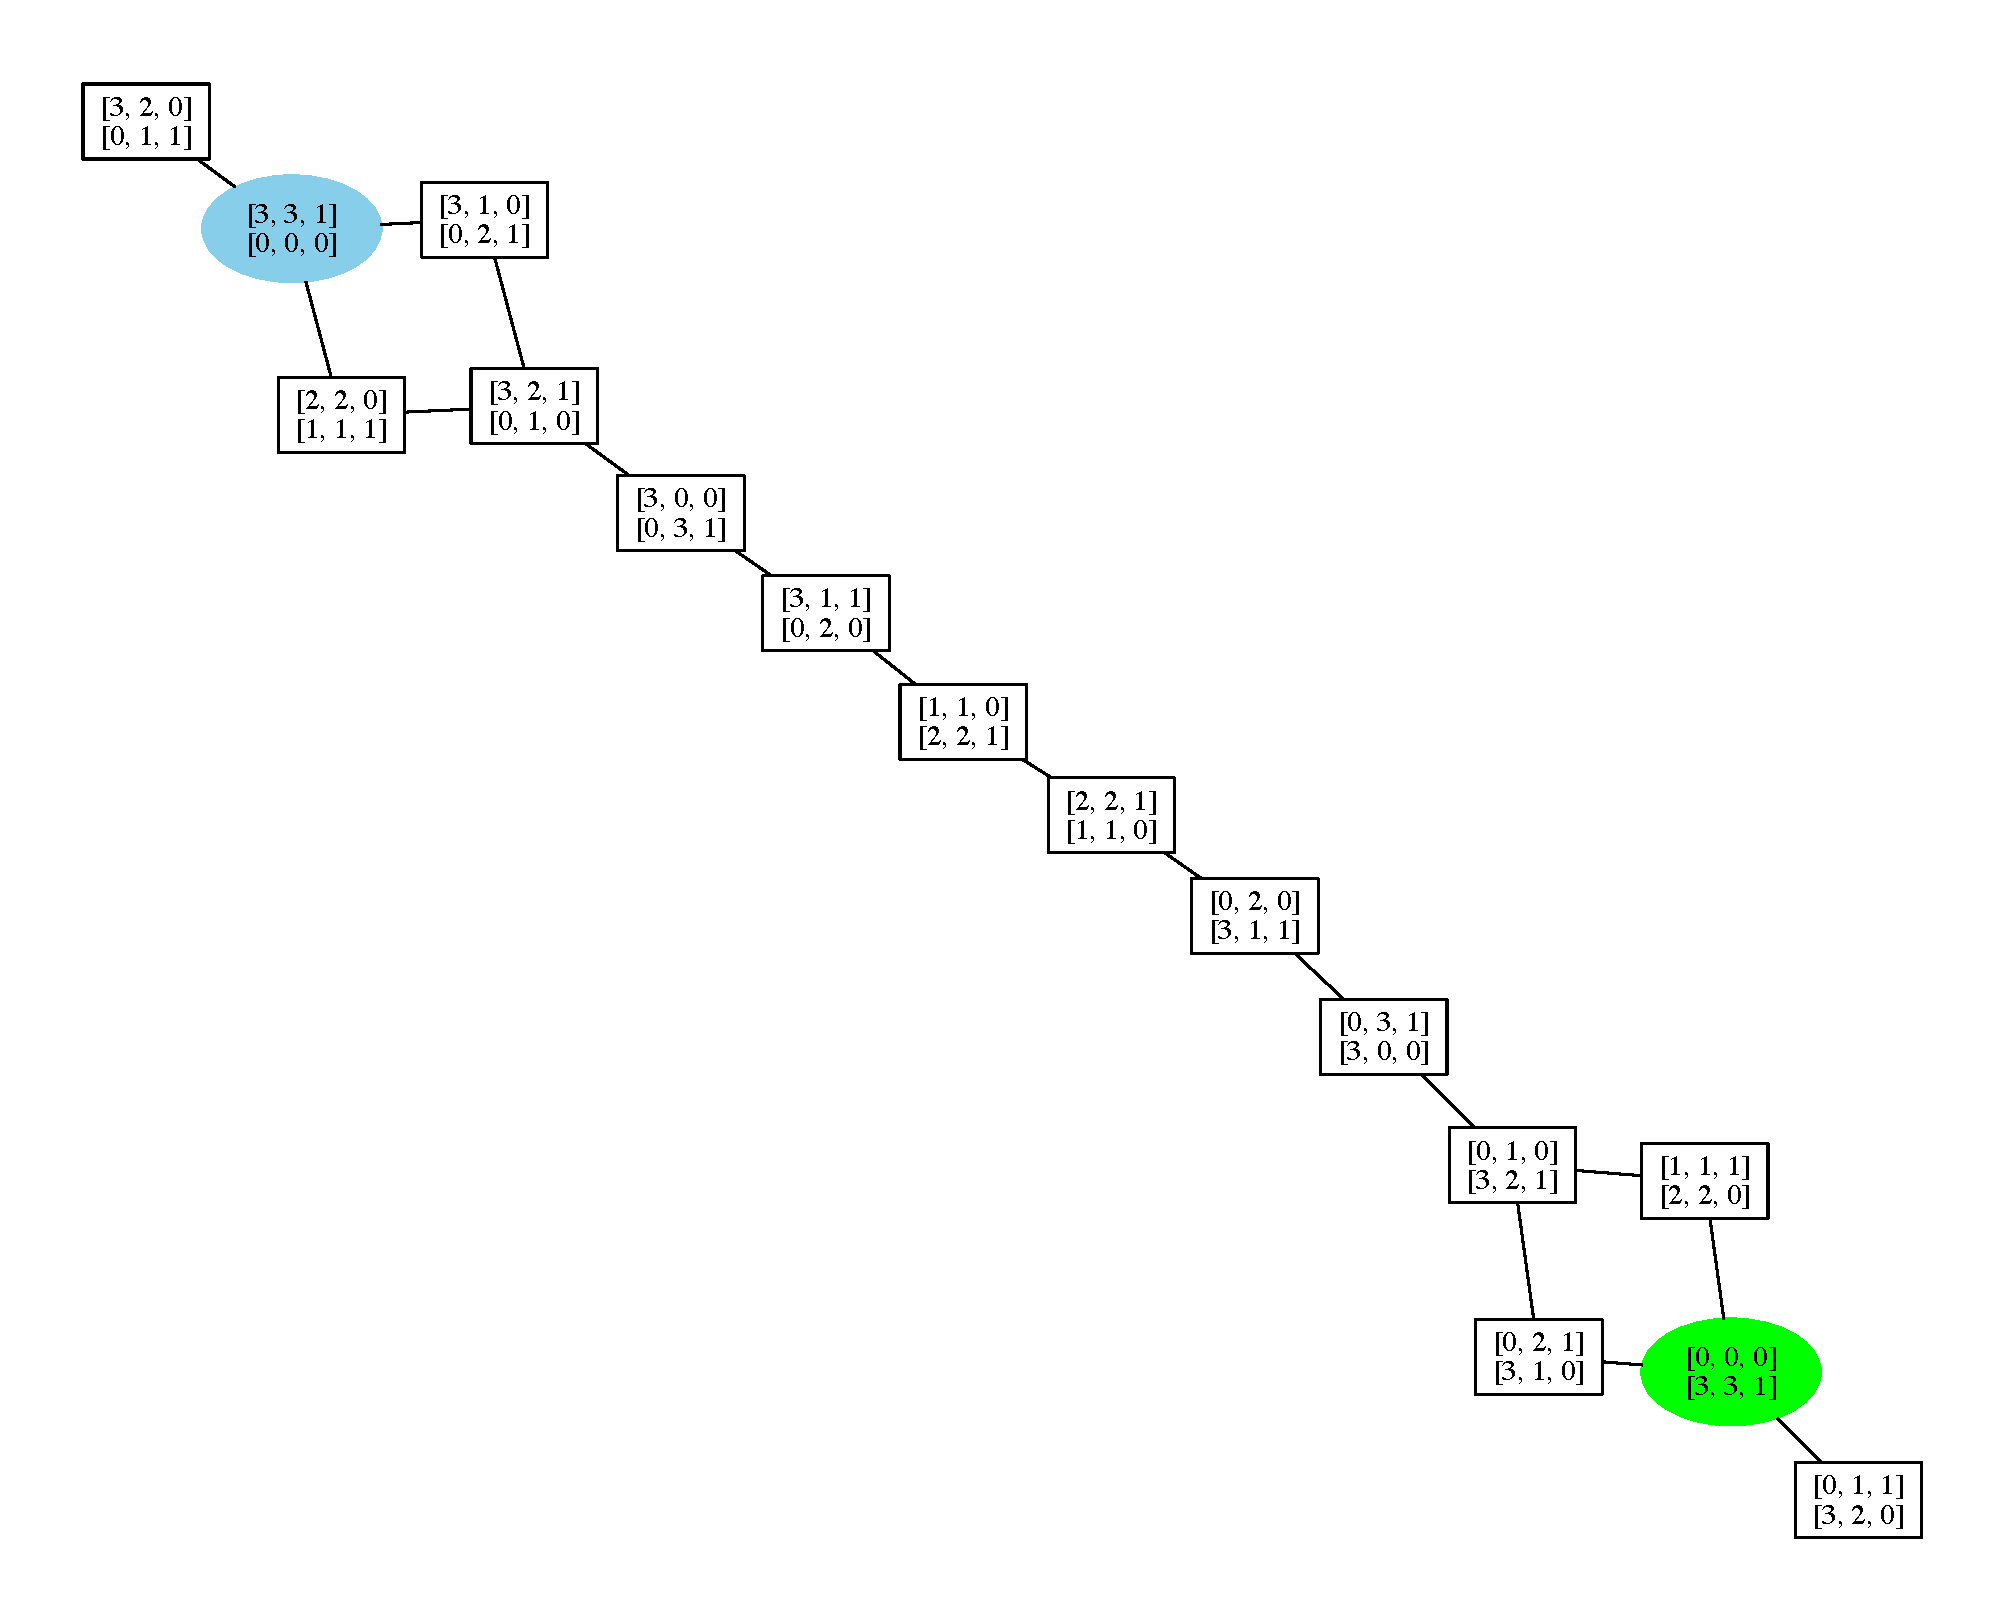
\epsfig{file=Figures/missionare.pdf,scale=0.5}} 
  \caption{A graphical representation of the missionaries and cannibals problem.}
  \label{fig:missionaries.pdf}
\end{figure}


\section{The Sliding Puzzle} 
The $3 \times 3$ sliding puzzle uses a
square board of length 3.  This board is subdivided into $3 \times 3 = 9$ squares of length 1.  Of
these 9 squares, 8 are occupied with square tiles that are numbered from 1 to 8.  One square remains
empty. Figure \ref{fig:8-puzzle.pdf} on page \ref{fig:8-puzzle.pdf} shows two possible states of this
sliding puzzle.  The $4 \times 4$ \href{https://en.wikipedia.org/wiki/15_puzzle}{sliding puzzle}
is similar to the $3 \times 3$ sliding puzzle but it is played on a square board of length 4
instead.  The $4 \times 4$ sliding puzzle is also known as the \emph{\color{blue}15 puzzle}, while the $3 \times 3$ puzzle is
called the \emph{\color{blue}8 puzzle}.

\begin{figure}[!ht]
\centering
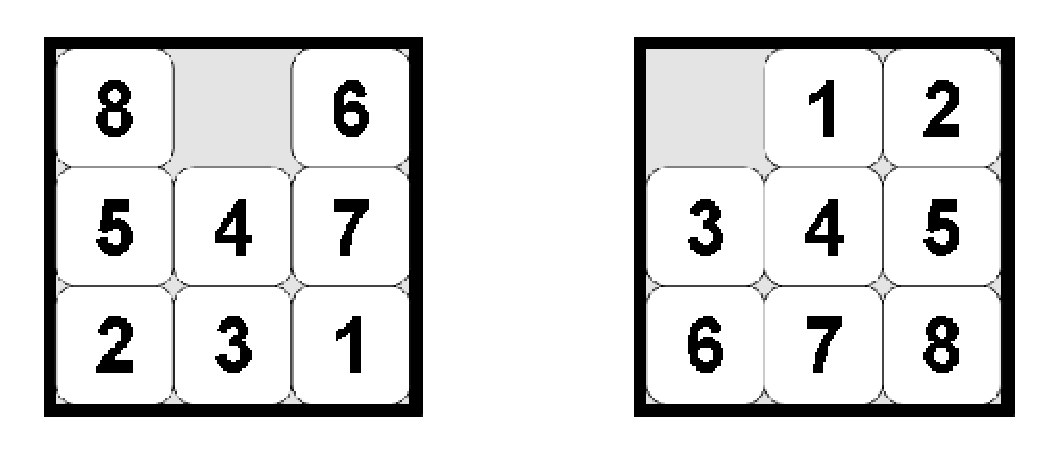
\epsfig{file=Figures/8-puzzle.pdf, scale=0.6}  
\caption{The $3 \times 3$ sliding puzzle.}
\label{fig:8-puzzle.pdf}
\end{figure}

In order to solve the $3 \times 3$ sliding puzzle shown in Figure \ref{fig:8-puzzle.pdf} we have to
transform the state shown on the left of Figure \ref{fig:8-puzzle.pdf} into the state shown on the
right of this figure.  The following operations are permitted when transforming a state of the
sliding puzzle:
\begin{enumerate}
\item If a tile is to the left  of the free square, this tile can be moved to the right.
\item If a tile is to the right of the free square, this tile can be moved to the left.
\item If a tile is above           the free square, this tile can be moved down.
\item If a tile is below           the free square, this tile can be moved up.
\end{enumerate}
In order to get a feeling for the complexity of the sliding puzzle, you can check the page
\\[0.2cm]
\hspace*{1.3cm}
\href{http://mypuzzle.org/sliding}{http://mypuzzle.org/sliding}.
\\[0.2cm]
The sliding puzzle is much more complex than the missionaries and cannibals problem because the
state space is much larger.  For the case of the $3 \times 3$ sliding puzzle, there are 9 squares
that can be positioned in $9!$ different ways.  It turns out that only half of these positions are
reachable from a given start state.  Therefore, the effective number of states for the $3 \times 3$
sliding puzzle is
\\[0.2cm]
\hspace*{1.3cm}
$9! / 2 = 181,440$.
\\[0.2cm]
This is already a big number, but $181,440$ states can still be stored in a modern computer.  However, the
$4 \times 4$ sliding puzzle has
\\[0.2cm]
\hspace*{1.3cm}
$16!/2 = 10,461,394,944,000$
\\[0.2cm]
different states reachable from a given start state.  If a state is represented as matrix containing
16 numbers and we store every number using just 4 bits, we still need $16 \cdot 4 = 64$ bits or 8
bytes for every state.  Hence we would need a total of
\\[0.2cm]
\hspace*{1.3cm}
$16! / 2 \cdots 8 = 83,691,159,552,000$
\\[0.2cm]
bytes to store every state. We would thus need about 84 Terabytes to store the set of all states.  As few
computers are equipped with this kind of memory, it is obvious that we won't be able to store the
entire state space in memory.

\begin{figure}[!ht]
\centering
\begin{Verbatim}[ frame         = lines, 
                  framesep      = 0.3cm, 
                  firstnumber   = 1,
                  labelposition = bottomline,
                  numbers       = left,
                  numbersep     = -0.2cm,
                  xleftmargin   = 0.8cm,
                  xrightmargin  = 0.8cm,
                ]
    findTile := procedure(number, state) {
        n := #state;
        L := [1 .. n]; 
        for (row in L, col in L | state[row][col] == number) {
            return [row, col];
        }
    };
    moveDir := procedure(state, row, col, dx, dy) {
        state[row     ][col     ] := state[row + dx][col + dy];
        state[row + dx][col + dy] := 0;
        return state;
    };
    nextStates := procedure(state) {
        n          := #state;
        [row, col] := findTile(0, state);
        newStates  := [];
        directions := [ [1, 0], [-1, 0], [0, 1], [0, -1] ];
        L          := [1 .. n];
        for ([dx, dy] in directions) {
            if (row + dx in L && col + dy in L) {
                newStates += [ moveDir(state, row, col, dx, dy) ];
            }
        }
        return newStates;
    };
    start := [ [8, 0, 6],
               [5, 4, 7],
               [2, 3, 1]
             ];
    goal := [ [0, 1, 2], 
              [3, 4, 5], 
              [6, 7, 8]
            ];
\end{Verbatim}
\vspace*{-0.3cm}
\caption{The $3 \times 3$ sliding puzzle.}
\label{fig:sliding-puzzle.stlx}
\end{figure}
Figure \ref{fig:sliding-puzzle.stlx} shows how the $3 \times 3$ sliding puzzle can be formulated as
a search problem.  We discuss this program line by line.
\begin{enumerate}
\item $\mathtt{findTile}$ is an auxiliary procedure that takes a $\mathtt{number}$ and a $\mathtt{state}$ and
      returns the row and column where the tile labeled with $\mathtt{number}$ can be found.  

      Here, a state is represented as a list of lists.  For example, the states shown in Figure
      \ref{fig:8-puzzle.pdf} are represented as shown in line 26 and line 30.  The empty tile is
      coded as $0$. 
\item $\mathtt{moveDir}$ takes a $\mathtt{state}$, the $\mathtt{row}$ and the $\mathtt{col}$umn
      where to find the empty square and a direction in which the empty square should be moved.
      This direction is specified via the two variables $\mathtt{dx}$ and $\mathtt{dy}$.  The tile
      at the position $\langle\mathtt{row} + \mathtt{dx}, \mathtt{col} + \mathtt{dy}\rangle$ is
      moved into the position $\langle\mathtt{row}, \mathtt{col}\rangle$, while the tile at position
      $\langle\mathtt{row} + \mathtt{dx}, \mathtt{col} + \mathtt{dy}\rangle$ becomes empty.
\item Given a $\mathtt{state}$, the procedure $\mathtt{newStates}$ computes the set of all states
      that can be reached in one step from $\mathtt{state}$.  The basic idea is to find the position of the
      empty tile and then try to move the empty tile in all possible directions.  If the empty tile is found at
      position $[\mathtt{row}, \mathtt{col}]$ and the direction of the movement is given as $[\mathtt{dx}, \mathtt{dy}]$, then
      in order to ensure that the empty tile can be moved to the position $[\mathtt{row}+\mathtt{dx}, \mathtt{col}+\mathtt{dy}]$,
      we have to ensure that both
      \\[0.2cm]
      \hspace*{1.3cm}
      $\mathtt{row}+\mathtt{dx} \in \{1,\cdots,n\}$ \quad and \quad
      $\mathtt{col}+\mathtt{dy} \in \{1,\cdots,n\}$
      \\[0.2cm]
      hold, where $n$ is the size of the board.
\end{enumerate}

Next, we want to develop an algorithm that can solve puzzles of the kind described so far.  The most basic
algorithm to solve search problems is \href{https://en.wikipedia.org/wiki/Breadth-first_search}{breadth first search}. 
We discuss this algorithm next.

\section{Breadth First Search}
Informally, breadth first search, abbreviated as \textsc{Bfs}, works as as follows:
\begin{enumerate}
\item Given a search problems $\langle Q,\mathtt{nextStates}, \mathtt{start}, \mathtt{goal}\rangle$,  
      we initialize a set $\mathtt{Frontier}$ to contain the state $\mathtt{start}$.

      In general, $\mathtt{Frontier}$ contains those states that have just been discovered and whose successors have not
      yet been seen.
\item As long as the set $\mathtt{Frontier}$ does not contain the state $\mathtt{goal}$, we recompute this set 
      by adding all states to it that can be reached in step from a state in $\mathtt{Frontier}$.
      Then, the states that had been previously present in $\mathtt{Frontier}$ are removed.
      These old states are then saved into a set $\mathtt{Visited}$.
\end{enumerate}
In order to avoid loops, an implementation of breadth first search keeps track of those states that have
been visited.  These states a collected in a set $\mathtt{Visited}$.  Once a state has been added to
the set $\mathtt{Visited}$,  it will never be revisited again. 
Furthermore, in order to keep track of the path leading to the goal, we have a dictionary
$\mathtt{Parent}$.  For every state $s$ that is in $\mathtt{Frontier}$, $\mathtt{Parent}[s]$ is the state that
caused $s$ to be added to the set $\mathtt{Frontier}$, i.e.~we have
\\[0.2cm]
\hspace*{1.3cm}
$s \in \mathtt{nextStates}(\mathtt{Parent}[s])$.


\begin{figure}[!ht]
\centering
\begin{Verbatim}[ frame         = lines, 
                  framesep      = 0.3cm, 
                  firstnumber   = 1,
                  labelposition = bottomline,
                  numbers       = left,
                  numbersep     = -0.2cm,
                  xleftmargin   = 0.8cm,
                  xrightmargin  = 0.8cm,
                ]
    search := procedure(start, goal, nextStates) {
        Frontier := { start };
        Visited  := {}; // set of nodes that have been expanded
        Parent   := {};
        while (Frontier != {}) {
            NewFrontier := {};
            for (s in Frontier, ns in nextStates(s) | !(ns in Visited)) {
                NewFrontier += { ns };
                Parent[ns]  := s;
                if (ns == goal) {
                    return pathTo(goal, Parent);
                }
            }
            Visited  += Frontier;
            Frontier := NewFrontier;
        }
    };
\end{Verbatim}
\vspace*{-0.3cm}
\caption{Breadth first search.}
\label{fig:breadth-first-search.stlx}
\end{figure}
\myFig{breadth-first-search.stlx} shows an implementation of
breadth first search in \textsc{SetlX}.  We discuss this implementation line by line:
\begin{enumerate}
\item $\mathtt{Frontier}$ is the set of all those states that have been encountered but whose
      neighbours have not yet been explored.  Initially, it contains the state $\mathtt{start}$.
\item $\mathtt{Visited}$ is the set of all those states, all whose neighbours have already been
      added to the set $\mathtt{Frontier}$.  In order to avoid infinite loops, these states must not
      be visited again.
\item $\mathtt{Parent}$ is a dictionary keeping track of the state leading to a given state.
\item As long as the set $\mathtt{Frontier}$ is not empty, we add all neighbours of states in 
      $\mathtt{Frontier}$ that have not yet been visited to the set $\mathtt{NewFrontier}$.
      When doing this, we keep track of the path leading to a new state $\mathtt{ns}$ by storing its
      parent in the dictionary $\mathtt{Parent}$.
\item If the new state happens to be the state $\mathtt{goal}$, we return a path leading from
      $\mathtt{start}$ to $\mathtt{goal}$.  The procedure $\mathtt{pathTo}()$ is shown in Figure
      \ref{fig:pathTo.stlx} on page \pageref{fig:pathTo.stlx}.
\item After we have collected all successors of states in $\mathtt{Frontier}$, the states
      in the set $\mathtt{Frontier}$ have been visited and are therefore added to the set
      $\mathtt{Visited}$, while the $\mathtt{Frontier}$ is updated to $\mathtt{NewFrontier}$.
\end{enumerate}

\begin{figure}[!ht]
\centering
\begin{Verbatim}[ frame         = lines, 
                  framesep      = 0.3cm, 
                  firstnumber   = 1,
                  labelposition = bottomline,
                  numbers       = left,
                  numbersep     = -0.2cm,
                  xleftmargin   = 0.8cm,
                  xrightmargin  = 0.8cm,
                ]
    pathTo := procedure(state, Parent) {
        Path := [];
        while (state != om) {
            Path  += [state];
            state := Parent[state];
        }
        return reverse(Path);
    };
\end{Verbatim}
\vspace*{-0.3cm}
\caption{The procedure $\mathtt{pathTo}()$.}
\label{fig:pathTo.stlx}
\end{figure}
The procedure call $\mathtt{pathTo}(\mathtt{state}, \mathtt{Parent})$ constructs a path reaching
from $\mathtt{start}$ to $\mathtt{state}$ in reverse by looking up the parent states.

If we try breadth first search to solve the missionaries and cannibals problem, we immediately get
the solution shown in Figure \ref{fig:missionaries.solution}.  15 nodes had to be expanded to find
this solution.  To keep this in perspective, we note that Figure \ref{fig:missionaries.pdf} shows
that the entire state space contains 16 states.  Therefore, with the exception of one state, we have
inspected all the states.  This is a typical behaviour for breadth first search.

\begin{figure}[!ht]
\centering
\begin{Verbatim}[ frame         = lines, 
                  framesep      = 0.3cm, 
                  firstnumber   = 1,
                  labelposition = bottomline,
                  numbers       = left,
                  numbersep     = -0.2cm,
                  xleftmargin   = 0.8cm,
                  xrightmargin  = 0.8cm,
                ]
    MMM   KKK   B      |~~~~~|                   
                       >  KK >
    MMM   K            |~~~~~|              KK  B
                       <  K  <
    MMM   KK    B      |~~~~~|               K   
                       >  KK >
    MMM                |~~~~~|             KKK  B
                       <  K  <
    MMM   K     B      |~~~~~|              KK   
                       > MM  >
    M     K            |~~~~~|        MM    KK  B
                       < M K <
    MM    KK    B      |~~~~~|         M     K   
                       > MM  >
          KK           |~~~~~|       MMM     K  B
                       <  K  <
          KKK   B      |~~~~~|       MMM         
                       >  KK >
          K            |~~~~~|       MMM    KK  B
                       <  K  <
          KK    B      |~~~~~|       MMM     K   
                       >  KK >
                       |~~~~~|       MMM   KKK  B
\end{Verbatim}
\vspace*{-0.3cm}
\caption{A solution of the missionaries and cannibals problem.}
\label{fig:missionaries.solution}
\end{figure}

Next, let us try to solve the $3 \times 3$ sliding puzzle.  It takes less about 9 seconds to solve
this problem on my computer\footnote{
  I happen to own an iMac from 2011.  This iMac is equipped with 16 Gigabytes of main memory and a
  quad core 2.7 GHz ``Intel Core i5'' processor.  I suspect this to be the I5-2500S (Sandy Bridge) processor.
}, while 181439 states are touched.  Again, we see that breadth first search touches nearly all the
states reachable from the start state.

\subsection{A Queue Based Implementation of Breadth First Search}
In the literature, for example in Figure 3.11 of Russell \& Norvig \cite{russell:2009}, breadth
first search is often implemented using a
\href{https://en.wikipedia.org/wiki/Queue_(abstract_data_type)}{queue} data structure.  
Figure \ref{fig:breadth-first-search-queue.stlx} on page
\pageref{fig:breadth-first-search-queue.stlx} shows an implementation of breadth first search that
uses a queue to store the set \texttt{Frontier}.  However, when we run this version, it turns out
that the solution of the $3 \times 3$ sliding puzzle needs about 94 seconds, which is more than
10 times slower than our set based implementation that has been presented in Figure
\ref{fig:breadth-first-search.stlx}.

\begin{figure}[!ht]
\centering
\begin{Verbatim}[ frame         = lines, 
                  framesep      = 0.3cm, 
                  firstnumber   = 1,
                  labelposition = bottomline,
                  numbers       = left,
                  numbersep     = -0.2cm,
                  xleftmargin   = 0.8cm,
                  xrightmargin  = 0.8cm,
                ]
    search := procedure(start, goal, nextStates) {
        Queue   := [ start ];
        Visited := {}; 
        Parent  := {};
        while (Queue != []) {
            state := Queue[1];
            Queue := Queue[2..];
            if (state == goal) {
                return pathTo(state, Parent);
            }
            if (state in Visited) {
                continue;
            }
            Visited   += { state };
            newStates := nextStates(state);
            for (ns in newStates | !(ns in Visited)) { 
                Parent[ns] := state;
                Queue      += [ ns ];
            }
        }
    };
\end{Verbatim}
\vspace*{-0.3cm}
\caption{A queue based implementation of breadth first search.}
\label{fig:breadth-first-search-queue.stlx}
\end{figure}

The solution of the $3 \times 3$ sliding puzzle that is found by breadth first search is shown in
Figure \ref{fig:8-puzzle.solution1} and Figure \ref{fig:8-puzzle.solution2}.

\begin{figure}[!ht]
\centering
\begin{Verbatim}[ frame         = lines, 
                  framesep      = 0.3cm, 
                  firstnumber   = 1,
                  labelposition = bottomline,
                  numbers       = left,
                  numbersep     = -0.2cm,
                  xleftmargin   = 0.8cm,
                  xrightmargin  = 0.8cm,
                ]
    +---+---+---+        +---+---+---+        +---+---+---+        +---+---+---+
    | 8 |   | 6 |        |   | 8 | 6 |        | 5 | 8 | 6 |        | 5 | 8 | 6 |
    +---+---+---+        +---+---+---+        +---+---+---+        +---+---+---+
    | 5 | 4 | 7 |  |==>  | 5 | 4 | 7 |  |==>  |   | 4 | 7 |  |==>  | 2 | 4 | 7 |  |==>
    +---+---+---+        +---+---+---+        +---+---+---+        +---+---+---+
    | 2 | 3 | 1 |        | 2 | 3 | 1 |        | 2 | 3 | 1 |        |   | 3 | 1 |
    +---+---+---+        +---+---+---+        +---+---+---+        +---+---+---+

    +---+---+---+        +---+---+---+        +---+---+---+        +---+---+---+
    | 5 | 8 | 6 |        | 5 | 8 | 6 |        | 5 | 8 | 6 |        | 5 | 8 |   |
    +---+---+---+        +---+---+---+        +---+---+---+        +---+---+---+
    | 2 | 4 | 7 |  |==>  | 2 | 4 | 7 |  |==>  | 2 | 4 |   |  |==>  | 2 | 4 | 6 |  |==>
    +---+---+---+        +---+---+---+        +---+---+---+        +---+---+---+
    | 3 |   | 1 |        | 3 | 1 |   |        | 3 | 1 | 7 |        | 3 | 1 | 7 |
    +---+---+---+        +---+---+---+        +---+---+---+        +---+---+---+

    +---+---+---+        +---+---+---+        +---+---+---+        +---+---+---+
    | 5 |   | 8 |        |   | 5 | 8 |        | 2 | 5 | 8 |        | 2 | 5 | 8 |
    +---+---+---+        +---+---+---+        +---+---+---+        +---+---+---+
    | 2 | 4 | 6 |  |==>  | 2 | 4 | 6 |  |==>  |   | 4 | 6 |  |==>  | 4 |   | 6 |  |==>
    +---+---+---+        +---+---+---+        +---+---+---+        +---+---+---+
    | 3 | 1 | 7 |        | 3 | 1 | 7 |        | 3 | 1 | 7 |        | 3 | 1 | 7 |
    +---+---+---+        +---+---+---+        +---+---+---+        +---+---+---+

    +---+---+---+        +---+---+---+        +---+---+---+        +---+---+---+
    | 2 | 5 | 8 |        | 2 | 5 | 8 |        | 2 | 5 | 8 |        | 2 | 5 |   |
    +---+---+---+        +---+---+---+        +---+---+---+        +---+---+---+
    | 4 | 1 | 6 |  |==>  | 4 | 1 | 6 |  |==>  | 4 | 1 |   |  |==>  | 4 | 1 | 8 |  |==>
    +---+---+---+        +---+---+---+        +---+---+---+        +---+---+---+
    | 3 |   | 7 |        | 3 | 7 |   |        | 3 | 7 | 6 |        | 3 | 7 | 6 |
    +---+---+---+        +---+---+---+        +---+---+---+        +---+---+---+

    +---+---+---+        +---+---+---+        +---+---+---+        +---+---+---+        
    | 2 |   | 5 |        |   | 2 | 5 |        | 4 | 2 | 5 |        | 4 | 2 | 5 |
    +---+---+---+        +---+---+---+        +---+---+---+        +---+---+---+
    | 4 | 1 | 8 |  |==>  | 4 | 1 | 8 |  |==>  |   | 1 | 8 |  |==>  | 1 |   | 8 |  |==>
    +---+---+---+        +---+---+---+        +---+---+---+        +---+---+---+
    | 3 | 7 | 6 |        | 3 | 7 | 6 |        | 3 | 7 | 6 |        | 3 | 7 | 6 |
    +---+---+---+        +---+---+---+        +---+---+---+        +---+---+---+

    +---+---+---+        +---+---+---+        +---+---+---+        +---+---+---+        
    | 4 | 2 | 5 |        | 4 | 2 | 5 |        | 4 | 2 | 5 |        | 4 | 2 |   |
    +---+---+---+        +---+---+---+        +---+---+---+        +---+---+---+
    | 1 | 7 | 8 |  |==>  | 1 | 7 | 8 |  |==>  | 1 | 7 |   |  |==>  | 1 | 7 | 5 |  |==>
    +---+---+---+        +---+---+---+        +---+---+---+        +---+---+---+
    | 3 |   | 6 |        | 3 | 6 |   |        | 3 | 6 | 8 |        | 3 | 6 | 8 |
    +---+---+---+        +---+---+---+        +---+---+---+        +---+---+---+
\end{Verbatim}
\vspace*{-0.3cm}
\caption{The first 24 steps in the solution of the $3 \times 3$ sliding puzzle.}
\label{fig:8-puzzle.solution1}
\end{figure}

\begin{figure}[!ht]
\centering
\begin{Verbatim}[ frame         = lines, 
                  framesep      = 0.3cm, 
                  firstnumber   = 1,
                  labelposition = bottomline,
                  numbers       = left,
                  numbersep     = -0.2cm,
                  xleftmargin   = 0.8cm,
                  xrightmargin  = 0.8cm,
                ]
    +---+---+---+        +---+---+---+        +---+---+---+        +---+---+---+        
    | 4 |   | 2 |        |   | 4 | 2 |        | 1 | 4 | 2 |        | 1 | 4 | 2 |
    +---+---+---+        +---+---+---+        +---+---+---+        +---+---+---+
    | 1 | 7 | 5 |  |==>  | 1 | 7 | 5 |  |==>  |   | 7 | 5 |  |==>  | 3 | 7 | 5 |  |==>
    +---+---+---+        +---+---+---+        +---+---+---+        +---+---+---+
    | 3 | 6 | 8 |        | 3 | 6 | 8 |        | 3 | 6 | 8 |        |   | 6 | 8 |
    +---+---+---+        +---+---+---+        +---+---+---+        +---+---+---+

    +---+---+---+        +---+---+---+        +---+---+---+        +---+---+---+        
    | 1 | 4 | 2 |        | 1 | 4 | 2 |        | 1 |   | 2 |        |   | 1 | 2 |
    +---+---+---+        +---+---+---+        +---+---+---+        +---+---+---+
    | 3 | 7 | 5 |  |==>  | 3 |   | 5 |  |==>  | 3 | 4 | 5 |  |==>  | 3 | 4 | 5 |  
    +---+---+---+        +---+---+---+        +---+---+---+        +---+---+---+
    | 6 |   | 8 |        | 6 | 7 | 8 |        | 6 | 7 | 8 |        | 6 | 7 | 8 |
    +---+---+---+        +---+---+---+        +---+---+---+        +---+---+---+
\end{Verbatim}
\vspace*{-0.3cm}
\caption{The last 7 steps in the solution of the $3 \times 3$ sliding puzzle.}
\label{fig:8-puzzle.solution2}
\end{figure}

We conclude our discussion of breadth first search by noting the two most important properties of
breadth first search.
\begin{enumerate}
\item Breadth first search is \emph{\color{blue}complete}:  If there is a solution to the given
      search problem, then breadth first search is going to find it.
\item The solution found by breadth first search is \emph{\color{blue}optimal}, i.e.~it is the
      shortest possible solution.
\end{enumerate}
\proof
Both of these claims can be shown simultaneously.  Consider the implementation of breadth first
search shown in Figure \ref{fig:breadth-first-search.stlx}.  An easy induction on the number of
iterations of the \texttt{while} loop shows that after $n$ iterations of the \texttt{while} loop,
the set $\mathtt{Frontier}$ contains exactly those states that have a distance of $n$ to the state 
$\mathtt{start}$.  This claim is obviously true before the first iteration of the while loop as in
this case, $\mathtt{Frontier}$ only contains the state $\mathtt{start}$.  In the induction step we
assume the claim is true after $n$ iterations.  Then, in the next iteration all states that can be
reached in one step from a state in $\mathtt{Frontier}$ are added to the new $\mathtt{Frontier}$,
provided there is no shorter path to these states.  There is a shorter path to these states if these
states are already a member of the set $\mathtt{Visited}$.  Hence, the claim is true after $n+1$
iterations also.

Now, if there is a path form $\mathtt{start}$ to $\mathtt{goal}$, there must also be a shortest
path.  Assume this path has a length of $k$.  Then, $\mathtt{goal}$ is reached in the iteration
number $k$ and the shortest path is returned.
\qed

The fact that breadth first search is both complete and the path returned is optimal is rather
satisfying.  However, breadth first search still has a big downside that makes it unusable for
many problems:  If the \texttt{goal} is far from the $\mathtt{start}$, breadth first search will use
a lot of memory because it will store a large part of the state space in the set
$\mathtt{Visited}$.  In many cases, the state space is so big that this is not possible.  For example, it is
impossible to solve the more interesting cases of the $4 \times 4$ sliding puzzle.

\section{Depth First Search}
To overcome the memory limitations of breadth first search, the
\href{https://en.wikipedia.org/wiki/Depth-first_search}{depth first search} algorithm has been
developed.  The basic idea is to replace the queue of Figure
\ref{fig:breadth-first-search-queue.stlx} by a stack.  The resulting algorithm is shown in Figure
\ref{fig:depth-first-search.stlx} on page \pageref{fig:depth-first-search.stlx}.  The basic idea is
to search a path up to its end before trying an alternative.  This way, we might be able to find a
$\mathtt{goal}$ that is far away from $\mathtt{start}$ without exploring the whole state space.  

\begin{figure}[!ht]
\centering
\begin{Verbatim}[ frame         = lines, 
                  framesep      = 0.3cm, 
                  firstnumber   = 1,
                  labelposition = bottomline,
                  numbers       = left,
                  numbersep     = -0.2cm,
                  xleftmargin   = 0.8cm,
                  xrightmargin  = 0.8cm,
                ]
    search := procedure(start, goal, nextStates) {
        Stack   := [ start ];
        Visited := {}; // number of nodes expanded
        Parent  := {};
        while (Stack != []) {
            state := Stack[-1];
            Stack := Stack[..-2];
            if (state == goal) {
                return pathTo(state, Parent);
            }
            if (state in Visited) {
                continue;
            }
            Visited   += { state };
            newStates := nextStates(state);
            for (ns in newStates | !(ns in Visited)) { 
                Parent[ns] := state;
                Stack      += [ns];
            }
        }
    };
\end{Verbatim}
\vspace*{-0.3cm}
\caption{The depth first search algorithm.}
\label{fig:depth-first-search.stlx}
\end{figure}
When we test this idea with the $3 \times 3$ sliding puzzle, the solution is found in less than 2
seconds.  This is more than four times faster than breadth first search.  Furthermore, only 9569
states were explored.  However, the solution that is found has a length of 9355 steps!  As the
shortest path from $\mathtt{start}$ to $\mathtt{goal}$ has 31 steps, the solution found by depth
first search is highly redundant.  If this redundancy is not an issue, depth first search is good
choice as it is very easy to implement.  For example, this is the case if we just want to know
whether there is a path leading from $\mathtt{start}$ to $\mathtt{goal}$.  However, if we are
interested in computing the shortest path, then depth first search is not an option.

\subsection{A Recursive Implementation of Depth First Search}
Sometimes, the depth first search algorithm is presented as a recursive algorithm, since this leads
to an implementation that is slightly shorter and more easy to understand.  While this program works
just fine for small problems like the missionaries and cannibals problem, it does not work so well
for a problem of the size of the $3 \times 3$ sliding puzzle.  The reason is that each recursive
invocation of the function $\mathtt{dfs}$ needs to copy the parameters onto the stack.  As the number of
recursive calls is the same as the length of the path that is found and as this path is very long, 
the resulting overhead is prohibitive.

\begin{figure}[!ht]
\centering
\begin{Verbatim}[ frame         = lines, 
                  framesep      = 0.3cm, 
                  firstnumber   = 1,
                  labelposition = bottomline,
                  numbers       = left,
                  numbersep     = -0.2cm,
                  xleftmargin   = 0.8cm,
                  xrightmargin  = 0.8cm,
                ]
    search := procedure(start, goal, nextStates) {
        return dfs(start, goal, nextStates, {}, {});
    };
    dfs := procedure(state, goal, nextStates, rw Parent, rw Visited) {
        if (state == goal) {
            return pathTo(goal, Parent);
        }
        Visited   += { state };
        newStates := nextStates(state);
        for (ns in newStates | !(ns in Visited)) {
            Parent[ns] := state;
            result     := dfs(ns, goal, nextStates, Parent, Visited);
            if (result != om) {
                return result;
            }   
        }
    };
\end{Verbatim}
\vspace*{-0.3cm}
\caption{A recursive implementation of depth first search.}
\label{fig:depth-first-search-recursive.stlx}
\end{figure}

\section{Iterative Deepening}
The fact that depth first search took just 2 seconds to find a solution is very impressive.  The questions is
whether it might be possible to force depth first search to find the shortest solution.  The answer to this
question leads to an algorithm that is known as
\href{https://en.wikipedia.org/wiki/Iterative_deepening_depth-first_search}{iterative deepening}.  The main
idea behind iterative deepening is to run depth first with a \emph{\color{blue}depth limit} $d$.  This limit
enforces that a solution has at most a length of $d$.  If no solution is found at a depth of $d$, the new depth
$d+1$ can be tried next and the process can be continued until a solution is found.  The program shown in
Figure \ref{fig:iterative-deepening.stlx} on page \pageref{fig:iterative-deepening.stlx} implements this strategy.
We continue to discuss the details of this program.

\begin{figure}[!ht]
\centering
\begin{Verbatim}[ frame         = lines, 
                  framesep      = 0.3cm, 
                  firstnumber   = 1,
                  labelposition = bottomline,
                  numbers       = left,
                  numbersep     = -0.2cm,
                  xleftmargin   = 0.8cm,
                  xrightmargin  = 0.8cm,
                ]
    search := procedure(start, goal, nextStates) {
        limit := 1;
        while (true) {
            path := depthLimitedSearch(start, goal, nextStates, limit);
            if (path != om) {
                return path;
            }
            limit += 1;
        }
    };    
    depthLimitedSearch := procedure(start, goal, nextStates, limit) {
        Stack    := [ start ];
        Distance := { [start, 0] };  // What is the distance to start?
        Parent   := {};
        while (Stack != []) {
            state := Stack[-1];
            Stack := Stack[..-2];
            if (state == goal) {
                return pathTo(state, Parent);
            }
            ds := Distance[state];            // ds:  distance state 
            if (ds >= limit) {
                continue;
            }
            for (ns in nextStates(state)) {   // ns:  new state
                dns := Distance[ns];          // dns: distance new state
                if (dns != om && dns <= ds + 1) {
                    continue;
                }
                Distance[ns] := ds + 1;
                Parent[ns]   := state;
                if (!(ns in Stack)) {
                    Stack += [ns];
                }
            }
        }
    };
\end{Verbatim}
\vspace*{-0.3cm}
\caption{Iterative deepening implemented in \textsc{SetlX}.}
\label{fig:iterative-deepening.stlx}
\end{figure}

\begin{enumerate}
\item The procedure $\mathtt{search}$ initializes the variable $\mathtt{limit}$ to 1 and tries to find a solution
      to the search problem that has a length that is less than or equal to $\mathtt{limit}$.  If a solution is
      found, it is returned.  Otherwise, the variable $\mathtt{limit}$ is incremented by one and a new depth
      first search is started.  This process continues until either a solution is found or the sun rises in the
      west. 
\item The procedure $\mathtt{depthLimitedSearch}$ implements depth first search but takes care to compute only
      those paths that have a length of at most $\mathtt{limit}$.  The implementation shown in Figure
      \ref{fig:iterative-deepening.stlx} is stack based.
\item The stack is initialized to contain the state $\mathtt{start}$.
\item For every state that is encountered in our search, we need to keep track of the distance of this state to
      the state $\mathtt{start}$.  This distance is stored in the dictionary $\mathtt{Distance}$.  Initially,
      only the distance of the node $\mathtt{start}$ is known.  Of course, this node has a distance of $0$ to
      the node $\mathtt{start}$.
\item In contrast to the implementation of depth first search shown in Figure \ref{fig:depth-first-search.stlx}
      on page \pageref{fig:depth-first-search.stlx}, we do \underline{not} keep track of the nodes that have
      been visited.  Hence, there is no need for the variable $\mathtt{Visited}$.  The reason is that the depth
      limit already ensures that the function $\mathtt{dfs}$ does not loop.  Furthermore, it actually might be necessary to
      revisit a given state:  Suppose that there is a state $s$ and the current estimation of the distance of
      $s$ from $\mathtt{start}$ is $5$.  Assume further that we now revisit the state $s$ on a path that would have
      a length of only $3$.  Finally, assume that we are using a depth $\mathtt{limit}$ of $6$ and that there
      is a path of length $2$ from the state $s$ to the state $\mathtt{goal}$.  If we would then discard
      further exploration of $s$ on the grounds that we have explored all its neighbours, we would then not be
      able to find the path of length $5$ that connects $\mathtt{start}$ with $\mathtt{goal}$!
\item Next, the first $\mathtt{state}$ is removed from the stack.  If this $\mathtt{state}$ happens to be the
      $\mathtt{goal}$, a path has been found and is returned.
\item Otherwise, we check the distance $\mathtt{ds}$ of $\mathtt{state}$.  If this distance is as big as the
      $\mathtt{limit}$, then $\mathtt{state}$ can be discarded as we have already checked that it is not the goal.
\item Otherwise, the neighbours of $\mathtt{state}$ are computed.  For every neighbour $\mathtt{ns}$ of
      $\mathtt{state}$, we look up its distance $\mathtt{dns}$ from $\mathtt{start}$.
      Now there are two cases.
      \begin{enumerate}
      \item If $\mathtt{dns}$ is less than or equal to $\mathtt{ds} + 1$, then 
            there is no point in pursuing a path from $\mathtt{start}$ to $\mathtt{ns}$ that leads through
            $\mathtt{state}$, as this path would have a length that is at least as long as the path from
            $\mathtt{start}$ to $\mathtt{ns}$ that has already been found.
      \item If $\mathtt{dns}$ is either undefined or bigger than $\mathtt{ds} + 1$, then
            we have to update the distance of $\mathtt{ns}$.  Furthermore, if the state $\mathtt{ns}$ is not
            already present on the stack, we have to push it onto $\mathtt{Stack}$.
      \end{enumerate}
      As in the original implementation of the depth first algorithm, this is process is iterated until the
      stack is exhausted.
\end{enumerate}
When we run this program to solve the $3 \times 3$ sliding puzzle, the algorithm takes a little less than 5
minutes and visits $103,324$ states.  There are two reasons for this:
\begin{enumerate}
\item First, it is quite wasteful to run the search for a depth limit of $1$, $2$, $3$, $\cdots$ all the way up
      to 31.  Essentially, all the computations done with a limit less the $31$ are essentially wasted.
\item When performing  the computation for the limit of $30$, all states that have a distance form start that
      is less than or equal to $30$ have to be visited.  This amounts to visiting $181,438$ states, because there
      are only two states that have a distance of $31$ from $\mathtt{start}$.  Hence, nearly the entire
      state space is visited.
\end{enumerate}

\exercise 
If there is no solution, the implementation of iterative deepening that is shown in Figure
\ref{fig:iterative-deepening.stlx} does not terminate.  The reason is that the function $\mathtt{dfs}$ does not
distinguish whether it fails to find a solution because the depth limit is reached or because the $\mathtt{Stack}$ is
exhausted.  Improve the implementation so that it will always terminate provided the state space is finite.

\subsection{A Recursive Implementation of Iterative Deepening}
If we implement iterative deepening recursively, then we know that the call stack is bounded by the length of
the shortest solution.  As the excessive length of the stack was the main culprit for the weak performance of
our recursive implementation of depth first search, we can hope that a recursive implementation of iterative
deepening is less disappointing than our recursive implementation of depth first has been.
Figure \ref{fig:iterative-deepening-recursive.stlx} on page \pageref{fig:iterative-deepening-recursive.stlx}
shows a recursive implementation of iterative deepening.  This implementation has several nice features:


\begin{figure}[!ht]
\centering
\begin{Verbatim}[ frame         = lines, 
                  framesep      = 0.3cm, 
                  firstnumber   = 1,
                  labelposition = bottomline,
                  numbers       = left,
                  numbersep     = -0.2cm,
                  xleftmargin   = 0.8cm,
                  xrightmargin  = 0.8cm,
                ]
    search := procedure(start, goal, nextStates) {
        limit := 1;  
        while (true) {
            result := dfsLimited(start, goal, nextStates, [start], limit);
            if (result != om) {
                return result;
            }
            limit += 1;
        }
    };
    dfsLimited := procedure(state, goal, nextStates, Path, limit) {
        if (state == goal) {
            return Path;
        }
        if (limit == 0) {
            return;  // limit execceded
        }
        for (ns in nextStates(state) | !(ns in Path)) {
            result := dfsLimited(ns, goal, nextStates, Path + [ns], limit - 1);
            if (result != om) {
                return result;
            }   
        }
    };
\end{Verbatim}
\vspace*{-0.3cm}
\caption{A recursive implementation of iterative deepening.}
\label{fig:iterative-deepening-recursive.stlx}
\end{figure}
\begin{enumerate}
\item The path that is computed no longer requires the dictionary $\mathtt{Parent}$ as it is built
      incrementally in the argument $\mathtt{Path}$ of the procedure $\mathtt{dfsLimited}$.
\item Similarly, there is no longer a need to keep the dictionary $\mathtt{Distance}$.
\end{enumerate}
Unfortunately, the running time of the recursive implementation of iterative deepening is still considerably
bigger than the running time of the stack based implementation:  On my computer, the recursive implementation
takes about 36 minutes!

\section{Bidirectional Breadth First Search}
The way breadth first search works it first visits all states that have a distance of 1 from start, then all
states that have a distance of 2, then of 3 and so on until finally the goal is found.  If the shortest path
from $\mathtt{start}$ to $\mathtt{goal}$ is $d$, then all states that have a distance of at most $d$ will be
generated.  In many search problems, the number of states grows exponentially with the distance. i.e.~there is
a \emph{\color{blue}branching factor} $b$ such that the set of all states that have a distance of at most $d$
from $\mathtt{start}$ is roughly
\\[0.2cm]
\hspace*{1.3cm}
 $\ds 1 + b + b^2 + b^3 + \cdots + b^d = \frac{b^{d+1} - 1}{b - 1} = \mathcal{O}\bigl(b^d\bigr)$. 
\\[0.2cm]
At least this is true in the beginning of the search.  As the size of
the memory that is needed is the most constraining factor when searching, it is important to cut down this
size.  On simple idea is to start searching both from the node $\mathtt{start}$ and the node $\mathtt{goal}$
simultaneously.  The justification is that we can hope that the path starting form $\mathtt{start}$ and the
path starting from $\mathtt{goal}$ will meet in the middle and hence will both have a size of approximately
$d/2$.  If this is the case, only
\\[0.2cm]
\hspace*{1.3cm}
$2 \cdot b^{d/2}$ 
\\[0.2cm]
nodes need to be explored and even for modest values of $b$ this number is much smaller than 
\\[0.2cm]
\hspace*{1.3cm}
$b^{d+1}$
\\[0.2cm]
which is the number of nodes expanded in breadth first search.  For example, assume that the branching factor
$b = 2$ and that the length of the shortest path leading from $\mathtt{start}$ to $\mathtt{goal}$
is $40$.  Then we need to explore
\\[0.2cm]
\hspace*{1.3cm}
$2^{40} = 1,099,511,627,776$
\\[0.2cm]
in breadth first search, while we only have to explore 
\\[0.2cm]
\hspace*{1.3cm}
$2^{40/2} = 1,048,576$
\\[0.2cm]
with bidirectional depth first search.  While it is certainly feasible to keep a million states in memory,
keeping a trillion states in memory is impossible on most average devices.


\begin{figure}[!ht]
\centering
\begin{Verbatim}[ frame         = lines, 
                  framesep      = 0.3cm, 
                  firstnumber   = 1,
                  labelposition = bottomline,
                  numbers       = left,
                  numbersep     = -0.2cm,
                  xleftmargin   = 0.8cm,
                  xrightmargin  = 0.8cm,
                ]
    search := procedure(start, goal, nextStates) {
        FrontierA := { start };
        VisitedA  := {}; // set of nodes expanded starting from start
        ParentA   := {};
        FrontierB := { goal };
        VisitedB  := {}; // set of nodes expanded starting from goal
        ParentB   := {};
        while (FrontierA != {} && FrontierB != {}) {
            VisitedA += FrontierA;
            VisitedB += FrontierB;
            NewFrontier := {};
            for (s in FrontierA, ns in nextStates(s) | !(ns in VisitedA)) {
                NewFrontier += { ns };
                ParentA[ns] := s;
                if (ns in VisitedB) {
                    return combinePaths(ns, ParentA, ParentB);
                }
            }
            FrontierA   := NewFrontier;
            NewFrontier := {};
            for (s in FrontierB, ns in nextStates(s) | !(ns in VisitedB)) {
                NewFrontier += { ns };
                ParentB[ns] := s;
                if (ns in VisitedA) {
                    return combinePaths(ns, ParentA, ParentB);
                }
            }
            FrontierB := NewFrontier;
        }
    };
\end{Verbatim}
\vspace*{-0.3cm}
\caption{Bidirectional breadth first search.}
\label{fig:bidirectional-bfs.stlx}
\end{figure}

Figure \ref{fig:bidirectional-bfs.stlx} on page \pageref{fig:bidirectional-bfs.stlx} shows the implementation
of bidirectional breadth first search.  Essentially, we have to keep to copy the breadth first program shown in
Figure \ref{fig:breadth-first-search.stlx}. Let us discuss the details of the implementation.
\begin{enumerate}
\item The variable $\mathtt{FrontierA}$ is the frontier that starts from the state $\mathtt{start}$, while
      $\mathtt{FrontierB}$ is the frontier that starts from the state $\mathtt{goal}$.
\item $\mathtt{VisitedA}$ is the set of states that have been visited starting from $\mathtt{start}$, while
      $\mathtt{VisitedB}$ is the set of states that have been visited starting from $\mathtt{goal}$.
\item For every state $s$ that is in $\mathtt{FrontierA}$, $\mathtt{ParentA}[s]$ is the state that caused $s$
      to be added to the set $\mathtt{FrontierA}$.  Similarly, for every state $s$ that is in $\mathtt{FrontierB}$,
      $\mathtt{ParentB}[s]$ is the state that caused $s$ to be added to the set $\mathtt{FrontierB}$.  
\item The bidirectional search keeps running for as long as both sets $\mathtt{FrontierA}$ and
      $\mathtt{FrontierB}$ are non-empty and a path has not yet been found.
\item Initially, the \texttt{while} loop adds the frontier sets to the visited sets
      as all the neighbours of the frontier sets will now be explored.
\item Then the \texttt{while} loop computes those states that can be reached from $\mathtt{FrontierA}$ and have not been
      visited from $\mathtt{start}$.  If a state $\mathtt{ns}$ is a neighbour of a state $\mathtt{s}$ from the set 
      $\mathtt{FrontierA}$ and the state $\mathtt{ns}$ has already been encountered during the search that started
      from $\mathtt{goal}$, then a path leading from $\mathtt{start}$ to $\mathtt{goal}$ has been found and this path
      is returned.  The function \texttt{combinePaths} that computes this path by combining the path that leads
      from $\mathtt{start}$ to $\mathtt{ns}$ and then from $\mathtt{ns}$ to $\mathtt{goal}$ to is shown in Figure
      \ref{fig:combine-paths.stlx} on page \pageref{fig:combine-paths.stlx}.
\item Next, the same computation is done with the role of the states $\mathtt{start}$ and $\mathtt{goal}$ exchanged.
\end{enumerate}
On my computer, bidirectional breadth first search solves the $3 \times 3$ sliding puzzle in less than a
second!  However, bidirectional breadth first search is still not able to solve the $4 \times 4$ sliding puzzle
since the portion of the search space that needs to be computed is still too big.

\begin{figure}[!ht]
\centering
\begin{Verbatim}[ frame         = lines, 
                  framesep      = 0.3cm, 
                  firstnumber   = 1,
                  labelposition = bottomline,
                  numbers       = left,
                  numbersep     = -0.2cm,
                  xleftmargin   = 0.8cm,
                  xrightmargin  = 0.8cm,
                ]
    combinePaths := procedure(node, ParentA, ParentB) {
        Path1 := pathTo(node, ParentA);
        Path2 := pathTo(node, ParentB);
        return Path1[..-2] + reverse(Path2);
    };
\end{Verbatim}
\vspace*{-0.3cm}
\caption{Combining two paths.}
\label{fig:combine-paths.stlx}
\end{figure}


\section{The A$^*$ Search Algorithm}
Up to now, all the search algorithms we have discussed were essentially blind.  Given a state $s$ and
all of its neighbours, they had no idea which of the neighbours they should pick because they had no conception
which of these neighbours might be more promising than the other neighbours.  If a human tries to solve a
problem, she usually will develop a feeling that certain states are more favourable than other states because
they seem to be closer to the solution.  In order to formalise this procedure, we next define the notion of a 
\emph{\color{blue}heuristic}.

\begin{Definition}[Heuristic]
Given a search problem
\\[0.2cm]
\hspace*{1.3cm}
$\mathcal{P} = \langle Q, \mathtt{nextStates}, \mathtt{start}, \mathtt{goal} \rangle$,
\\[0.2cm]
a \emph{\color{blue}heuristic} is a function
\\[0.2cm]
\hspace*{1.3cm}
$h: Q \rightarrow \mathbb{R}$
\\[0.2cm]
that computes an approximation of the distance of a given state $s$ to the goal state $\mathtt{goal}$.
The heuristic is \emph{\color{blue}admissible} if it always underestimates the true distance, i.e.~if the function
\\[0.2cm]
\hspace*{1.3cm}
$d:Q \rightarrow \mathbb{R}$
\\[0.2cm]
computes the true distance of a state $s$ to the goal, then we must have
\\[0.2cm]
\hspace*{1.3cm}
$h(s) \leq d(s)$ \quad for all $s \in Q$.
\\[0.2cm]
Hence, the heuristic is admissible iff it is optimistic:  An admissible heuristic must never overestimate the
distance to the goal, but it is free to underestimate this distance.

Finally, the  heuristic $h$ is called \emph{\color{blue}consistent} iff we have
\\[0.2cm]
\hspace*{1.3cm}
$h(\mathtt{goal}) = 0$ \quad and \quad $h(s_1) \leq 1 + h(s_2)$ \quad for all $s_2 \in \mathtt{neighbours}(s_1)$.  \eod
\end{Definition}

Let us explain the idea behind the notion of consistency.  First, if we are already at the goal, the heuristic
should notice this and hence return $h(\mathtt{goal}) = 0$.  Secondly, assume we are at the state $s_1$ and $s_2$ is a
neighbour of $s_1$, i.e.~we have that 
\\[0.2cm]
\hspace*{1.3cm}
$s_2 \in \mathtt{nextStates}(s_1)$.
\\[0.2cm]
Now if our heuristic $h$ assumes that the distance of $s_2$ from the $\mathtt{goal}$ is $h(s_2)$, then the distance of
$s_1$ from the $\mathtt{goal}$ can be at most $1 + h(s_2)$ because starting from $s_1$ we can first go to $s_2$
in one step and then from $s_2$ to $\mathtt{goal}$ in $h(s_2)$ steps for a total of $1 + h(s_2)$ steps.  Of
course, it is possible that there exists a cheaper path from $s_1$ leading to the $\mathtt{goal}$ than the one
that visits $s_2$ first.  Hence we have the inequality 
\\[0.2cm]
\hspace*{1.3cm}
$h(s_1) \leq 1 + h(s_2)$.

\begin{Theorem}
  Every consistent heuristic is also admissible. 
\end{Theorem}

\proof
Assume that the heuristic $h$ is consistent.  Assume further that $s \in Q$ is some state such that there is a
path $p$ from $s$ to the $\mathtt{goal}$.  Assume this path has the form
\\[0.2cm]
\hspace*{1.3cm}
$p = [s_n, s_{n-1}, \cdots, s_1, s_0]$, \quad where $s_n = s$ and $s_0 = \mathtt{goal}$.
\\[0.2cm]
Then the length of $p$ is $n$ and we have to show that $h(s) \leq n$.  In order to prove this claim, we show
that we have
\\[0.2cm]
\hspace*{1.3cm}
$h(s_k) \leq k$ \quad for all $k \in \{0, 1, \cdots, n\}$.
\\[0.2cm]
This claim is shown by induction on $k$.
\begin{enumerate}
\item[B.C.:] $k=0$.

             We have $h(s_0) = h(\mathtt{goal}) = 0 \leq 0$ because the fact that $h$ is consistent implies 
             $h(\mathtt{goal}) = 0$. 
\item[I.S.:] $k \mapsto k+1$.
  
             We have to show that $h(s_{k+1}) \leq k + 1$ holds.  This is shown as follows:
             \\[0.2cm]
             \hspace*{1.3cm}
             $
             \begin{array}{lcll}
               h(s_{k+1}) & \leq & 1 + h(s_k) & \mbox{because $h$ is consistent} \\[0.2cm]
                         & \leq & 1 + k      & \mbox{because $h(s_k) \leq k$ by i.h.}
             \end{array}
             $
             \\[0.2cm]
             This concludes the proof.  \qed
\end{enumerate}

It is natural to ask whether the last theorem can be reversed, i.e.~whether every admissible heuristic is also
consistent.  The answer to this question is negative since there are
\href{http://web.cs.du.edu/~sturtevant/papers/incnew.pdf}{some} \emph{\color{red}contorted}
heuristics that are admissible but that fail to be consistent.  However, in practice it turns out that most 
admissible heuristics are also consistent.  Therefore, when we construct consistent heuristics later, we will
start with admissible heuristics, since these are easy to find.  We will then have to check that these 
heuristics are also consistent.  

\examples
In the following, we will discuss several heuristics for the sliding puzzle. 
\begin{enumerate}
\item The simplest heuristic that is admissible is the function $h(s) := 0$.  Since we have
      \\[0.2cm]
      \hspace*{1.3cm}
      $0 \leq 1 + 0$,
      \\[0.2cm]
      this heuristic is obviously consistent, but this heuristic is too trivial to be of any use.
\item The next heuristic is the \emph{\color{blue}number of misplaced tiles} heuristic.  For a state $s$, 
      this heuristic counts the number of tiles in $s$ that are not in their final position, i.e.~that are not
      in the same position as the corresponding tile in $\mathtt{goal}$.  For example, in \myFig{8-puzzle.pdf}
      in the state depicted to the left, only the tile with the label $4$ is in the same
      position as in the state depicted to the right.  Hence, there are 7 misplaced tiles.

      As every misplaced tile must be moved at least once and every step in the sliding puzzle moves at most
      one tile, it is obvious that this heuristic is admissible.  It is also consistent.  First, the
      $\mathtt{goal}$ has no misplaced tiles, hence its heuristic is $0$.  Second, in every step of the sliding
      puzzle  only one tile is moved.  Therefore the number of misplaced tiles in two neighbouring state can
      differ by at most one.

      We will later see that the number of misplaced tiles heuristic is very crude and therefore not
      particularly useful.
\item The \emph{\color{blue}Manhattan heuristic} improves on the previous heuristic.  For two points 
      $\pair(x_1, y_1), \pair(x_2, y_2) \in \mathbb{R}^2$ the \emph{\color{blue}Manhattan distance} of these
      points is defined as 
      \\[0.2cm]
      \hspace*{1.3cm}
      $d_1\bigl(\langle x_1, y_1\rangle, \langle x_2, y_2\rangle\bigr) := |x_1 - x_2| + |y_1 - y_2|$.
      \\[0.2cm]
      If we associate coordinates
      \href{https://en.wikipedia.org/wiki/Cartesian_coordinate_system}{Cartesian coordinates} with
      the tiles of the sliding puzzle such that the tile in the upper left corner has coordinates
      $\pair(1, 1)$ and the coordinates of the tile in the lower right corner is $\pair(3, 3)$, then
      the Manhattan distance of two positions measures how many steps it takes to move a tile from
      the first position to the second position if we are only allowed to move the tile horizontally
      or vertically.  To compute the Manhattan heuristic for a state $s$ with respect to the
      $\mathtt{goal}$, we first define the position $\mathtt{pos}(t, s)$ for all tiles 
      $t \in \{1,\cdots, 8\}$ in a given state $s$ as follows:
      \\[0.2cm]
      \hspace*{1.3cm}
      $\mathtt{pos}(t, s) = \pair(\mathtt{row}, \mathtt{col}) 
         \;\stackrel{\mathrm{def}}{\Longleftrightarrow}\; s[\mathtt{row}][\mathtt{col}] = t
      $,
      \\[0.2cm]
      i.e.~given a state $s$, the expression $\mathtt{pos}(t, s)$ computes the Cartesian coordinates of
      the tile $t$ with respect to $s$.  Then we can define the Manhattan heuristic $h$ for the $3 \times 3$ puzzle
      as follows:  
      \\[0.2cm]
      \hspace*{1.3cm}
      $\ds h(s) := \sum\limits_{t=1}^8 d_1\bigl(\mathtt{pos}(t,s),\, \mathtt{pos}(t, \mathtt{goal})\bigr)$.
      \\[0.2cm]
      The Manhattan heuristic measure the number of moves that would be needed if we wanted to put every tile
      of $s$ into its final positions and if we were allowed to slide tiles over each other.  Figure
      \ref{fig:manhattan.stlx} on page \pageref{fig:manhattan.stlx} shows how the Manhattan distance can be
      computed.  The code given in that figure works for a general $n \times n$ sliding puzzle.  It takes two
      states $\mathtt{stateA}$ and $\mathtt{stateB}$ and computes the Manhattan distance between these states.
      \begin{enumerate}
      \item First, the size $\mathtt{n}$ of the puzzle is computed by checking the number of rows of
            $\mathtt{stateA}$.
      \item Next, the \texttt{for} loop iterates over all rows and columns of $\mathtt{stateA}$ that do not 
            contain a blank tile.  Remember that the blank tile is coded using the number $0$.  The tile at
            position $\pair(\mathtt{rowA}, \mathtt{colA})$ in $\mathtt{stateA}$ is computed using the expression \texttt{stateA[rowA][colA]} and the
            corresponding position $\pair(\mathtt{rowB}, \mathtt{colB})$ of this tile in state $\mathtt{stateB}$ is computed using the function
            $\mathtt{findTile}$.
      \item Finally, the Manhattan distance between the two positions $\pair(\mathtt{rowA}, \mathtt{colA})$ and
            $\pair(\mathtt{rowB}, \mathtt{colB})$ is added to the $\mathtt{result}$.
      \end{enumerate}

      \begin{figure}[!ht]
        \centering
        \begin{Verbatim}[ frame         = lines, 
                          framesep      = 0.3cm, 
                          firstnumber   = 1,
                          labelposition = bottomline,
                          numbers       = left,
                          numbersep     = -0.2cm,
                          xleftmargin   = 0.8cm,
                          xrightmargin  = 0.8cm,
                        ]
    manhattan := procedure(stateA, stateB) {
        n := #stateA;
        L := [1 .. n];
        result := 0;
        for (rowA in L, colA in L | stateA[rowA][colA] != 0) {
            [rowB, colB] := findTile(stateA[rowA][colA], stateB);
            result += abs(rowA - rowB) + abs(colA - colB);
        }
        return result;
    };
    \end{Verbatim}
    \vspace*{-0.3cm}
    \caption{The Manhattan distance between two states.}
    \label{fig:manhattan.stlx}
    \end{figure}
    
    The Manhattan distance is admissible.  The reason is that if $s_2 \in \mathtt{nextStates}(s_1)$,
    then there can be only one tile $t$ such that the position of $t$ in $s_1$ is different from the position
    of $t$ in $s_2$.  Furthermore, this position differs by either one row or one column.  Therefore,
    \\[0.2cm]
    \hspace*{1.3cm}
    $|h(s_1) - h(s_2)| = 1$
    \\[0.2cm]
    and hence $h(s_1) \leq 1 + h(s_2)$.  \qed
\end{enumerate}
Now we are ready to describe how the $\mathrm{A}^*$ algorithm uses its heuristic.  The basic idea is that the
$\mathrm{A}^*$ search algorithm works similar to the queue based version of breadth first search, but instead
of using a simple queue, a priority queue is used instead.  The priority $f(s)$ of every state $s$ is given as
\\[0.2cm]
\hspace*{1.3cm}
$f(s) := g(s) + h(s)$,
\\[0.2cm]
where $g(s)$ computes the length of the path leading from $\mathtt{start}$ to $s$ and $h(s)$ is the heuristical
estimate of the distance from $s$ to $\mathtt{goal}$.  The details of the $\mathrm{A}^*$ algorithm are given in
\myFig{a-star-search.stlx} and discussed below.


\begin{figure}[!ht]
\centering
\begin{Verbatim}[ frame         = lines, 
                  framesep      = 0.3cm, 
                  firstnumber   = 1,
                  labelposition = bottomline,
                  numbers       = left,
                  numbersep     = -0.2cm,
                  xleftmargin   = 0.0cm,
                  xrightmargin  = 0.0cm,
                ]
    aStarSearch := procedure(start, goal, nextStates, heuristic) {
        Parent   := {};                    // back pointers, represented as dictionary
        Distance := { [start, 0] };
        estGoal  := heuristic(start, goal);
        Estimate := { [start, estGoal] };  // Estimated distance
        Frontier := { [estGoal, start] };  // priority queue
        while (Frontier != {}) {
            [stateEstimate, state] := fromB(Frontier);
            if (state == goal) {
                return pathTo(state, Parent);
            }
            stateDist := Distance[state];
            for (neighbour in nextStates(state)) {
                oldEstimate := Estimate[neighbour];
                newEstimate := stateDist + 1 + heuristic(neighbour, goal);
                if (oldEstimate == om || newEstimate < oldEstimate) {
                    Parent[neighbour]   := state;
                    Distance[neighbour] := stateDist + 1;
                    Estimate[neighbour] := newEstimate;
                    Frontier            += { [newEstimate, neighbour] };
                    if (oldEstimate != om) {
                        Frontier -= { [oldEstimate, neighbour] };
                    }
                }
            }
        }
    };
\end{Verbatim}
\vspace*{-0.3cm}
\caption{The A$^*$ search algorithm.}
\label{fig:a-star-search.stlx}
\end{figure}
\noindent
The function \texttt{aStarSearch} takes 4 parameters:
\begin{enumerate}
\item \texttt{start} is a state.  This state represents the start state of the search problem.
\item \texttt{goal} is the goal state.  
\item \texttt{next} is a function that takes a state as a parameter.  For a state $s$,
      \\[0.2cm]
      \hspace*{1.3cm}
      $\mathtt{next}(s)$
      \\[0.2cm]
      computes the set of all those states that can be reached from $s$ in a single step.
\item \texttt{heuristic} is a function that takes two parameters.  
      For two states $s_1$ and $s_2$, the expression
      \\[0.2cm]
      \hspace*{1.3cm}
      $\texttt{heuristic}(s_1, s_2)$ 
      \\[0.2cm]
      computes an estimate of the distance between $s_1$ and $s_2$.
\end{enumerate}
The function $\mathtt{aStarSearch}$ maintains 5 variables that are crucial for the understanding of the
algorithm. 
\begin{enumerate}
\item $\mathtt{Parent}$ is a dictionary associating a parent state with those states that have already been
      encountered during the search, i.e.~we have
      \\[0.2cm]
      \hspace*{1.3cm}
      $\mathtt{Parent}[s_2] = s_1 \;\Rightarrow\; s_2 \in \mathtt{nextStates}(s_1)$.
      \\[0.2cm]
      Once the goal has been found, this dictionary is used to compute the path from $\mathtt{start}$ to
      $\mathtt{goal}$. 
\item $\mathtt{Distance}$ is a dictionary that remembers for every state $s$ that is encountered during the
      search the length of the shortest path from $\mathtt{start}$ to $s$.
\item $\mathtt{Estimate}$ is a dictionary.  For every state $s$ encountered in the search, $\mathtt{Estimate}[s]$
      is an estimate of the length that a path from $\mathtt{start}$ to $\mathtt{goal}$ would have if it would
      pass through the state $s$.  This estimate is calculated using the equation
      \\[0.2cm]
      \hspace*{1.3cm}
      $\mathtt{Estimate}[s] = \mathtt{Distance}[s] + \mathtt{heuristic}(s, \mathtt{goal})$.
      \\[0.2cm]
      Instead of recalculating this sum every time we need it, we store it in the dictionary
      $\mathtt{Estimate}$.
\item $\mathtt{Frontier}$ is a \href{https://en.wikipedia.org/wiki/Priority_queue}{priority queue}.
      The elements of $\mathtt{Frontier}$ are pairs of the form
      \\[0.2cm]
      \hspace*{1.3cm}
      $[d, s]$ \quad such that \quad $d = \mathtt{Estimate}[s]$,
      \\[0.2cm]
      i.e.~if $[d, s] \in \mathtt{Frontier}$, then the state $s$ has been encountered in the search and it is
      estimated that a path leading from $\mathtt{start}$ to $\mathtt{goal}$ and passing through $s$ would have
      a length of $d$.
\end{enumerate}
Now that we have established the key variables, the $\mathrm{A}^*$ algorithm runs in a \texttt{while} loop that
does only terminate if either a solution is found or the priority queue $\mathtt{Frontier}$ is exhausted.
\begin{enumerate}
\item First, the $\mathtt{state}$ with the smallest estimated distance for a path running from $\mathtt{start}$
      to $\mathtt{goal}$ and passing through $\mathtt{state}$ is chosen from the priority queue
      $\mathtt{Frontier}$.  Note that the call to $\mathtt{fromB}$ does not only return the pair
      \\[0.2cm]
      \hspace*{1.3cm}
      $[\mathtt{stateEstimate}, \mathtt{state}]$
      \\[0.2cm]
      from $\mathtt{Frontier}$ that has the lowest value of $\mathtt{stateEstimate}$, but also removes this
      pair from the priority queue.
\item Now if this $\mathtt{state}$ is the $\mathtt{goal}$ a solution has been found and is returned.
\item Otherwise, we check the length of path leading from $\mathtt{start}$ to state.  This length is stored in 
      \texttt{stateDist}.  Effectively, this is the distance between $\mathtt{start}$ and $\mathtt{state}$.
\item Next, we have a loop that iterates over all neighbours of $\mathtt{state}$.
      \begin{enumerate}
      \item For every $\mathtt{neighbour}$ we check the estimated length of a solution passing through
            $\mathtt{neighbour}$ and store this length in $\mathtt{oldEstimate}$.   Note that
            $\mathtt{oldEstimate}$ is undefined, i.e.~$\mathtt{om}$ if we haven't yet encountered the node
            $\mathtt{neighbour}$ in our search.
      \item If a solution would go from $\mathtt{start}$ to $\mathtt{state}$ and from there proceed to
            $\mathtt{neighbour}$, the the estimated length of this solution would be
            \\[0.2cm]
            \hspace*{1.3cm}
            $\mathtt{stateDist} + 1 + \mathtt{heuristic}(\mathtt{neighbour}, \mathtt{goal})$.
            \\[0.2cm]
            Therefore this value is stored in $\mathtt{newEstimate}$.  
      \item Next, we need to check whether this new solution that first passes through $\mathtt{state}$ and
            then proceeds to $\mathtt{neighbour}$ is better than the previous solution that passes through
            $\mathtt{neighbour}$.  This check is done by comparing $\mathtt{newEstimate}$ and
            $\mathtt{oldEstimate}$.  Note that we have to take care of the fact that there might be no valid
            $\mathtt{oldEstimate}$.

            In case the new solution seems better than the old solution, we have to update
            the $\mathtt{Parent}$ dictionary, the $\mathtt{Distance}$ dictionary, and the $\mathtt{Estimate}$
            dictionary.  Furthermore we have to update the priority queue $\mathtt{Frontier}$.
      \end{enumerate}
\end{enumerate}
It can be shown that the $\mathrm{A}^*$ search algorithm is complete and that the computed solution is optimal.

When we run $\mathrm{A}^*$ on the $3 \times 3$ sliding puzzle, it takes about 17 seconds to solve the instance
shown in \myFig{8-puzzle.pdf}.  If we just look at the time, this seems to be disappointing.  However, the good
news is that now only $10\,061$ states are touched in the search for a solution.  This is more than a tenfold
reduction when compared with breadth first search.  The fact that the running time
is, nevertheless, quite high results from the complexity of computing the Manhattan distance.



\section{Bidirectional $\mathrm{A}^*$ Search}
\begin{figure}[!ht]
\centering
\begin{Verbatim}[ frame         = lines, 
                  framesep      = 0.3cm, 
                  firstnumber   = 1,
                  labelposition = bottomline,
                  numbers       = left,
                  numbersep     = -0.2cm,
                  xleftmargin   = 0.0cm,
                  xrightmargin  = 0.0cm,
                ]
    aStarSearch := procedure(start, goal, nextStates, heuristic) {
        ParentA    := {};                     ParentB    := {};                    
        DistanceA  := { [start, 0] };         DistanceB  := { [goal,  0] };
        estimate   := heuristic(start, goal);
        EstimateA  := { [start, estimate] };  EstimateB  := { [goal,  estimate] };  
        FrontierA  := { [estimate, start] };  FrontierB  := { [estimate, goal ] };  
        while (FrontierA != {} && FrontierB != {}) {
            [guessA, stateA] := first(FrontierA);
            stateADist       := DistanceA[stateA];
            [guessB, stateB] := first(FrontierB);
            stateBDist       := DistanceB[stateB];
            if (guessA <= guessB) {
                FrontierA -= { [guessA, stateA] };
                for (neighbour in nextStates(stateA)) {
                    oldEstimate := EstimateA[neighbour];
                    newEstimate := stateADist + 1 + heuristic(neighbour, goal);
                    if (oldEstimate == om || newEstimate < oldEstimate) {
                        ParentA[neighbour]   := stateA;
                        DistanceA[neighbour] := stateADist + 1;
                        EstimateA[neighbour] := newEstimate;
                        FrontierA            += { [newEstimate, neighbour] };
                        if (oldEstimate != om) { FrontierA -= { [oldEstimate, neighbour] }; }
                    }
                    if (DistanceB[neighbour] != om) {
                        return combinePaths(neighbour, ParentA, ParentB);
                    }
                }
            } else {
                FrontierB -= { [guessB, stateB] };
                for (neighbour in nextStates(stateB)) {
                    oldEstimate := EstimateB[neighbour];
                    newEstimate := stateBDist + 1 + heuristic(start, neighbour);
                    if (oldEstimate == om || newEstimate < oldEstimate) {
                        ParentB[neighbour]   := stateB;
                        DistanceB[neighbour] := stateBDist + 1;
                        EstimateB[neighbour] := newEstimate;
                        FrontierB            += { [newEstimate, neighbour] };
                        if (oldEstimate != om) { FrontierB -= { [oldEstimate, neighbour] }; }
                    }
                    if (DistanceA[neighbour] != om) {
                        return combinePaths(neighbour, ParentA, ParentB);
                    }
                }        
            }
        }
    };
\end{Verbatim}
\vspace*{-0.3cm}
\caption{Bidirectional $\mathrm{A}^*$ search.}
\label{fig:a-star-bidirectional.stlx}
\end{figure}
So far, the best search algorithm we have encountered is bidirectional breadth first search.  However, in terms
of memory consumption, the $\mathrm{A}^*$ algorithm also looks very promising.  Hence, it might be a good idea
to combine these two algorithms.  \myFig{a-star-bidirectional.stlx} shows the resulting program.  This program
relates to the $\mathrm{A}^*$ algorithm shown in \myFig{a-star-search.stlx} as the algorithm for bidirectional
search shown in \myFig{bidirectional-bfs.stlx} relates to breadth first search shown in \myFig{breadth-first-search.stlx}.
Hence, we will not discuss the details any further.

When we run bidirectional $\mathrm{A}^*$ search for the $3 \times 3$ sliding puzzle shown in
\myFig{8-puzzle.pdf}, the program takes 2 second but only uses $2,963$ states.  Therefore, I have tried 
to solve the $4 \times 4$ sliding puzzle shown in \myFig{start-goal.stlx} using
bidirectional $\mathrm{A}^*$ search.  A solution of $44$ steps was found in $65$ seconds.
Only $20,624$ states had to be processed to compute this solution!  None of the other algorithms presented so
far was able to compute the solution.

\begin{figure}[!ht]
\centering
\begin{Verbatim}[ frame         = lines, 
                  framesep      = 0.3cm, 
                  firstnumber   = 1,
                  labelposition = bottomline,
                  numbers       = left,
                  numbersep     = -0.2cm,
                  xleftmargin   = 0.8cm,
                  xrightmargin  = 0.8cm,
                ]
    start := [ [  1, 2,  0,  4 ],
               [ 14, 7, 12, 10 ],
               [  3, 5,  6, 13 ],
               [ 15, 9,  8, 11 ]
             ];
    goal  := [ [  1,  2,  3,  4 ],
               [  5,  6,  7,  8 ],
               [  9, 10, 11, 12 ],
               [ 13, 14, 15,  0 ]
             ];
\end{Verbatim}
\vspace*{-0.3cm}
\caption{A start state and a goal state for the $4 \times 4$ sliding puzzle.}
\label{fig:start-goal.stlx}
\end{figure}
\section{Iterative Deepening $\mathrm{A}^*$ Search}
So far, we have combined $\mathrm{A}^*$ search with bidirectional search and achieved good results.  When
memory space is too limited for bidirectional $\mathrm{A}^*$ search to be possible, we can instead
combine $\mathrm{A}^*$ search with \emph{iterative deepening}.  The resulting search technique is known as 
\href{https://en.wikipedia.org/wiki/Iterative_deepening_A*}{\color{blue}iterative deepening $\mathrm{A}^*$ search} 
and is commonly abbreviated as $\mathrm{IDA}^*$.   \myFig{iterative-deepening-a-star.stlx}
shows an implementation of $\mathrm{IDA}^*$ in \textsc{SetlX}.  We proceed to discuss this program.

\begin{figure}[!ht]
\centering
\begin{Verbatim}[ frame         = lines, 
                  framesep      = 0.3cm, 
                  firstnumber   = 1,
                  labelposition = bottomline,
                  numbers       = left,
                  numbersep     = -0.2cm,
                  xleftmargin   = 0.8cm,
                  xrightmargin  = 0.8cm,
                ]
    idaStarSearch := procedure(start, goal, nextStates, heuristic) {
        limit := heuristic(start, goal);
        while (true) {
            Path := search(start, goal, nextStates, 0, limit, [start], heuristic);
            if (isList(Path)) {
                return Path;
            }
            limit := Path;
        }
    };
    search := procedure(state, goal, nextStates, distance, limit, Path, heuristic) {
        total  := distance + heuristic(state, goal);
        if (total > limit) {
            return total;
        }
        if (state == goal) {
            return Path;
        }
        smallest := 1.0 / 0.0;  // infinity
        for (ns in nextStates(state) | !(ns in Path) ) {
            result := search(ns, goal, nextStates, distance + 1, limit, 
                             Path + [ ns ], heuristic);
            if (isList(result)) {
                return result;
            }
            if (result < smallest) {
                smallest := result;
            }
        }
        return smallest;
    };
\end{Verbatim}
\vspace*{-0.3cm}
\caption{Iterative deepening $A^*$ search.}
\label{fig:iterative-deepening-a-star.stlx}
\end{figure}
\begin{enumerate}
\item As in the $\mathrm{A}^*$ search algorithm, the function \texttt{idaStarSearch} takes four parameters.
      \begin{enumerate}
      \item \texttt{start} is a state.  This state represents the start state of the search problem.
      \item \texttt{goal} is the goal state.  
      \item \texttt{nextStates} is a function that takes a state $s$ as a parameter and 
            computes the set of all those states that can be reached from $s$ in a single step.
      \item \texttt{heuristic} is a function that takes two parameters $s_1$ and $s_2$, where $s_1$ and $s_2$
            are states. The expression
            \\[0.2cm]
            \hspace*{1.3cm}
            $\texttt{heuristic}(s_1, s_2)$ 
            \\[0.2cm]
            computes an estimate of the distance between $s_1$ and $s_2$.
     \end{enumerate}
\item The function \texttt{idaStarSearch} initialises $\mathtt{limit}$ to be an estimate of the distance
      between $\mathtt{start}$ and $\mathtt{goal}$.  As we assume that the function $\mathtt{heuristic}$ is
      optimistic, we know that there is no path from $\mathtt{start}$ to $\mathtt{goal}$ that is shorter than
      $\mathtt{limit}$.  Hence, we start our search by assuming that we might find a path that has a length of 
      $\mathtt{limit}$.
\item Next, we start a loop.  In this loop, we call the function $\mathtt{search}$ to compute a path from
      $\mathtt{start}$ to $\mathtt{goal}$ that has a length of at most $\mathtt{limit}$.  This function
      $\mathtt{search}$ uses $\mathrm{A}^*$ search and is described in detail below.
      Now there are two cases:
      \begin{enumerate}
      \item $\mathtt{search}$ does find a path.  In this case, this path is returned in the variable
            $\mathrm{Path}$ and this variable is a list.  This list is returned as the solution to the search
            problem.
      \item $\mathtt{search}$ is not able to find a path within the given $\mathtt{limit}$.  In this case,
            $\mathrm{search}$ will not return a path but instead it will return a number.  This number will
            specify the minimal length that any path leading from $\mathtt{start}$ to $\mathtt{goal}$ needs to
            have.  This number is then used to update the $\mathtt{limit}$ which is used for the next
            invocation of $\mathtt{search}$.

            \textbf{Note} that the fact that $\mathtt{search}$ is able to compute this new $\mathtt{limit}$ is
            a significant enhancement of iterative deepening.  While we had to test every single possible
            length in iterative deepening, now the fact that we can intelligently update the $\mathtt{limit}$
            results in a considerable saving of computation time.
      \end{enumerate}
\end{enumerate}
We proceed to discuss the function \texttt{search}. This function takes 7 parameters, which we describe next.
\begin{enumerate}
\item $\mathtt{state}$ is a state.  Initially, $\mathtt{state}$ is the $\mathtt{start}$ state.  However,
      on recursive invocations of $\mathtt{search}$, $\mathtt{state}$ is some state such that we have already
      found a path from $\mathtt{start}$ to $\mathtt{state}$.
\item $\mathtt{goal}$ is another state.  The purpose of the recursive invocations of $\mathtt{search}$ is to
      find a path from $\mathtt{state}$ to $\mathtt{goal}$.
\item $\mathtt{nextStates}$ is a function that takes a state $s$ as input and computes the set of states that are
      reachable from $s$ in one step. 
\item $\mathtt{distance}$ is the distance between  $\mathtt{start}$ and $\mathtt{state}$.  It is also the
      length of the list $\mathtt{Path}$ described below.
\item $\mathtt{limit}$ is the maximal length of the path from $\mathtt{start}$ to $\mathtt{goal}$.
\item $\mathtt{Path}$ is a path from $\mathtt{start}$ to $\mathtt{state}$.
\item $\texttt{heuristic}(s_1, s_2)$ computes an \emph{estimate} of the distance between $s_1$ and $s_2$.  It is
      assumed that this estimate is optimistic, i.e.~the value returned by $\mathtt{heuristic}(s_1, s_2)$ 
      is less or equal than the true distance between $s_1$ and $s_2$.
\end{enumerate}
We proceed to describe the implementation of the function \texttt{search}.
\begin{enumerate}
\item As $\mathtt{distance}$ is the length of $\mathtt{Path}$ and the $\mathrm{heuristic}$ is assumed to be optimistic,
      i.e.~it always underestimates the true distance, if we want to extend $\mathtt{Path}$, then the best we
      can hope for is to find a path from $\mathtt{start}$ to $\mathtt{goal}$ that has a length of
      \\[0.2cm]
      \hspace*{1.3cm}
      $\mathtt{distance} + \mathtt{heuristic}(\mathtt{state}, \mathtt{goal})$.
      \\[0.2cm]
      This length is computed and saved in the variable $\mathtt{total}$.
\item If $\mathtt{total}$ is bigger than $\mathtt{limit}$, it is not possible to find a path from
      $\mathtt{start}$ to $\mathtt{goal}$ passing through $\mathtt{state}$ that has a length of at most
      $\mathtt{limit}$.  Hence, in this case we return $\mathtt{total}$ to communicate that the limit needs to
      be increased to have at least a value of $\mathtt{total}$.
\item If we are lucky and have found the $\mathtt{goal}$, the $\mathtt{Path}$ is returned.
\item Otherwise, we iterate over all nodes reachable from $\mathtt{state}$ that have not already been visited
      by $\mathtt{Path}$.  If $\mathtt{ns}$ is a a node of this kind, we extend the $\mathtt{Path}$ so that
      this node is visited next.  The resulting path is 
      \\[0.2cm]
      \hspace*{1.3cm}
      \texttt{Path + [ ns ]}.
      \\[0.2cm]
      Next, we recursively start a new search starting from the node $\mathtt{ns}$.  If this search is
      successful, the resulting path is returned.  Otherwise, the search returns the minimum distance that is
      needed to reach the state $\mathtt{goal}$ from the state $\mathtt{ns}$.  If this distance is smaller than
      the distance returned from previous nodes which is stored in the variable $\mathtt{smallest}$, this
      variable is updated accordingly.  This way, if the $\mathtt{for}$ loop is not able to return a path
      leading to $\mathtt{goal}$, the variable $\mathtt{smallest}$ contains the minimum distance that is needed
      to reach $\mathtt{goal}$ by a path that extends the given $\mathtt{Path}$.
      
      \textbf{Note}: At this point, a natural question is to ask whether the $\mathtt{for}$ loop should collect
      all paths leading to $\mathtt{goal}$ and then only return that path that is shortest.  However, this is
      not necessary:  Every time the function $\mathtt{search}$ is invoked it is already guaranteed that there
      is no path that is shorter than the parameter $\mathtt{limit}$.  Therefore, if $\mathtt{search}$ is able
      to find a path that has a length of at most $\mathtt{limit}$, this path is already know to be optimal.
\end{enumerate}
Iterative deepening $\mathrm{A}^*$ is a complete search algorithm that does find an optimal path, provided that the employed heuristic
is optimistic.  On the instance of the $3 \times 3$ sliding puzzle shown on \myFig{8-puzzle.pdf}, this
algorithm takes about $2.6$ seconds to solve the puzzle.  For the $4 \times 4$ sliding puzzle, the algorithm
takes about $518$ seconds.  Although this is more than the time needed by bidirectional $\mathrm{A}^*$ search,
the good news is that the $\mathrm{IDA}^*$ algorithm does not need much memory since basically only the path
discovered so far is stored in memory.  Hence, $\mathrm{IDA}^*$ is a viable alternative if the available memory
does is not sufficient for the bidirectional $\mathrm{A}^*$ algorithm.

\section{The $\mathrm{A}^*$-$\mathrm{IDA}^*$ Search Algorithm}
So far, from all of the algorithms we have tried, the bidirectional $\mathrm{A}^*$ search has performed best.  However,
bidirectional $\mathrm{A}^*$ search is only feasible if sufficient memory is available.   While
$\mathrm{IDA}^*$ does take longer, its memory consumption is much lower than the memory consumption of
bidirectional $\mathrm{A}^*$.  Hence, it is natural to try to combine these two algorithms.  Concretely, the
idea is to run an $\mathrm{A}^*$ search from the $\mathrm{start}$ node until memory is more or less
exhausted.  Then, we start $\mathrm{IDA}^*$ form the $\mathrm{goal}$ node and search until we find any of the
nodes discovered by the $\mathrm{A}^*$ search that has been started from the $\mathrm{start}$ node.

\begin{figure}[!ht]
\centering
\begin{Verbatim}[ frame         = lines, 
                  framesep      = 0.3cm, 
                  firstnumber   = 1,
                  labelposition = bottomline,
                  numbers       = left,
                  numbersep     = -0.2cm,
                  xleftmargin   = 0.8cm,
                  xrightmargin  = 0.8cm,
                ]
    aStarIdaStarSearch := procedure(start, goal, nextStates, heuristic, size) {
        Parent   := {};
        Distance := { [start, 0] };
        est      := heuristic(start, goal);
        Estimate := { [start, est] };  
        Frontier := { [est, start] };
        while (#Distance < size && Frontier != {}) {
            [guess, state] := first(Frontier);
            if (state == goal) {
                return pathTo(state, Parent);
            }
            stateDist := Distance[state];
            Frontier  -= { [guess, state] };
            for (neighbour in nextStates(state)) {
                oldEstimate := Estimate[neighbour];
                newEstimate := stateDist + 1 + heuristic(neighbour, goal);
                if (oldEstimate == om || newEstimate < oldEstimate) {
                    Parent[neighbour]   := state;
                    Distance[neighbour] := stateDist + 1;
                    Estimate[neighbour] := newEstimate;
                    Frontier            += { [newEstimate, neighbour] };
                    if (oldEstimate != om) {
                        Frontier -= { [oldEstimate, neighbour] };
                    }
                }
            }
        }
        [s, P] := deepeningSearch(goal, start, nextStates, heuristic, Distance);
        return pathTo(s, Parent) + P;
    };
\end{Verbatim}
\vspace*{-0.3cm}
\caption{The $\mathrm{A}^*$-$\mathrm{IDA}^*$ search algorithm, part \texttt{I}.}
\label{fig:a-star-ida-star.stlx-1}
\end{figure}

An implementation of the $\mathrm{A}^*$-$\mathrm{IDA}^*$ algorithm is shown in \myFig{a-star-ida-star.stlx-1}
and \myFig{a-star-ida-star.stlx-2}.  We begin with a discussion of the procedure $\mathtt{aStarIdaStarSearch}$.
\begin{enumerate}
\item The procedure takes 5 arguments.
      \begin{enumerate}[(a)]
      \item $\mathtt{start}$ and $\mathtt{goal}$ are nodes.  The procedure tries to find a path connecting 
            $\mathtt{start}$ and $\mathtt{goal}$.
      \item $\mathtt{nextStates}$ is a function that takes a state $s$ as input and computes the set of states that are
            reachable from $s$ in one step. 
      \item $\mathtt{heuristic}$ computes an \emph{estimate} of the distance between $s_1$ and $s_2$.  It is
            assumed that this estimate is optimistic, i.e.~the value returned by $\mathtt{heuristic}(s_1, s_2)$ 
            is less or equal than the true distance between $s_1$ and $s_2$.
      \item $\mathtt{size}$ is the maximal number of states that the $\mathrm{A}^*$ search is allowed to
            explore before the algorithm switches over to $\mathrm{IDA}^*$ search.
      \end{enumerate}
\item The basic idea behind the $\mathrm{A}^*$-$\mathrm{IDA}^*$ algorithm is to first use $\mathrm{A}^*$ search
      to find a path from $\mathrm{start}$ to $\mathtt{goal}$.  If this is successfully done without visiting
      more than $\mathrm{size}$ nodes, the algorithm terminates and returns the path that has been found.  
      Otherwise, the algorithm switches over to an $\mathrm{IDA}^*$ search that starts from $\mathtt{goal}$ and
      tries to connect goal to any of the nodes that have been encountered during the $\mathrm{A}^*$ search.
      To this end, the procedure $\mathtt{aStarIdaStarSearch}$ maintains the following variables.
      \begin{enumerate}
      \item $\mathtt{Parent}$ is a dictionary associating a parent state with those states that have already been
            encountered during the search, i.e.~we have
            \\[0.2cm]
            \hspace*{1.3cm}
            $\mathtt{Parent}[s_2] = s_1 \;\Rightarrow\; s_2 \in \mathtt{nextStates}(s_1)$.
            \\[0.2cm]
            Once the goal has been found, this dictionary is used to compute the path from $\mathtt{start}$ to
            $\mathtt{goal}$. 
      \item $\mathtt{Distance}$ is a dictionary that remembers for every state $s$ that is encountered during the
            $\mathrm{A}^*$ search the length of the shortest path from $\mathtt{start}$ to $s$.
      \item $\mathtt{Estimate}$ is a dictionary.  For every state $s$ encountered in the $\mathrm{A}^*$ search, $\mathtt{Estimate}[s]$
            is an estimate of the length that a path from $\mathtt{start}$ to $\mathtt{goal}$ would have if it would
            pass through the state $s$.  This estimate is calculated using the equation
            \\[0.2cm]
            \hspace*{1.3cm}
            $\mathtt{Estimate}[s] = \mathtt{Distance}[s] + \mathtt{heuristic}(s, \mathtt{goal})$.
            \\[0.2cm]
            Instead of recalculating this sum every time we need it, we store it in the dictionary
            $\mathtt{Estimate}$.
      \item $\mathtt{Frontier}$ is a \href{https://en.wikipedia.org/wiki/Priority_queue}{priority queue}.
            The elements of $\mathtt{Frontier}$ are pairs of the form
            \\[0.2cm]
            \hspace*{1.3cm}
            $[d, s]$ \quad such that \quad $d = \mathtt{Estimate}[s]$,
            \\[0.2cm]
            i.e.~if $[d, s] \in \mathtt{Frontier}$, then the state $s$ has been encountered in the $\mathrm{A}^*$ search and it is
            estimated that a path leading from $\mathtt{start}$ to $\mathtt{goal}$ and passing through $s$ would have
            a length of $d$.
      \end{enumerate}
\item The $\mathrm{A}^*$ search runs exactly as discussed previously.  The only difference is that the
      \texttt{while} loop is terminated once the dictionary $\mathtt{Distance}$ has more than $\mathtt{size}$
      entries.  If we are lucky, the $\mathrm{A}^*$ search is already able to find the $\mathrm{goal}$ and the
      algorithm terminates.
\item Otherwise, the procedure $\mathtt{deepeningSearch}$ is called.  This procedure starts an iterative deepening
      $\mathrm{A}^*$ search from the node $\mathtt{goal}$.  This search terminates as soon as a state is found
      that has already been encountered during the $\mathrm{A}^*$ search.  The set of these nodes is given to
      the procedure $\mathtt{deepeningSearch}$ via the parameter $\mathrm{Distance}$.  The procedure
      $\mathtt{deepeningSearch}$ returns a pair.  The first component of this pair is the state $s$.  This is
      the state in $\mathtt{Distance}$ that has been reached by the $\mathrm{IDA}^*$ search.  The second component is the
      path $P$ that leads from the node $s$ to the node $\mathrm{goal}$ but that does not include the node $s$.
      In order to compute a path from $\mathtt{start}$ to $\mathtt{goal}$, we still have to compute a
      path from $\mathtt{start}$ to $s$.  This path is then combined with the path $P$ and the resulting path
      is returned.
\end{enumerate}


\begin{figure}[!ht]
\centering
\begin{Verbatim}[ frame         = lines, 
                  framesep      = 0.3cm, 
                  firstnumber   = 1,
                  labelposition = bottomline,
                  numbers       = left,
                  numbersep     = -0.2cm,
                  xleftmargin   = 0.8cm,
                  xrightmargin  = 0.8cm,
                ]
    deepeningSearch := procedure(g, s, nextStates, heuristic, Distance) {
        limit := 0;
        while (true) {
            Path := search(g, s, nextStates, 0, limit, heuristic, [g], Distance);
            if (isList(Path)) {
                return Path;
            }
            limit := Path;
        }
    };
    search := procedure(g, s, nextStates, d, l, heuristic, Path, Dist) {
        total := d + heuristic(g, s);
        if (total > l) {
            return total;
        }
        if (Dist[g] != om) {
            return [g, Path[2..]];
        }
        smallest := 1.0 / 0.0;  // infinity
        for (ns in nextStates(g) | !(ns in Path)) {
            result := search(ns, s, nextStates, d+1, l, heuristic, [ns]+Path, Dist);
            if (isList(result)) {
                return result;
            }
            if (result < smallest) {
                smallest := result;
            }
        }
        return smallest;
    };
\end{Verbatim}
\vspace*{-0.3cm}
\caption{The $\mathrm{A}^*$-$\mathrm{IDA}^*$ search algorithm, part \texttt{II}.}
\label{fig:a-star-ida-star.stlx-2}
\end{figure}

Iterative deepening $\mathrm{A}^*$-$\mathrm{IDA}^*$ is a complete search algorithm. 
On the instance of the $3 \times 3$ sliding puzzle shown on \myFig{8-puzzle.pdf}, this
algorithm takes about $1.4$ seconds to solve the puzzle.  For the $4 \times 4$ sliding puzzle, if the algorithm
is allowed to visit at most $3\,000$ states, the algorithm takes less than $9$ seconds.  However, there is one
caveat: $\mathrm{A}^*$-$\mathrm{IDA}^*$ search is not \emph{guaranteed} to find an optimal path, although in practise it often does. 

\exercise
Assume that you have 3 water buckets:  The first bucket can hold 12 liters of water, the second bucket can hold 8 liters,
while the last bucket can hold 3 liters.  There are three types of action:
\begin{enumerate}
\item A bucket can be completely filled.
\item A bucket can be completely emptied.
\item The contend of one bucket can be poured into another bucket.  Then, there are two cases.
      \begin{enumerate}[(a)]
      \item If the second bucket has enough free space for all the water in the first bucket, 
            then the first bucket is emptied and all the water from the first bucket is poured 
            into the second bucket.  
      \item However, if there is not enough space in the second bucket, then the second bucket is filled
            completely, while the water that does not fit into the second bucket remains in the first bucket.  
      \end{enumerate}
\end{enumerate}
Your goal is to measure out exactly one liter.  Write a program that computes a plan to achieve this goal.
\eox


%%% Local Variables:
%%% mode: latex
%%% TeX-master: "artificial-intelligence"
%%% End:
